\chapter{Estudo de Caso: Atividades 2 e 3} \label{Chap:AppendixLesson2}

\section{Atividade 2: Plano de Aula}\label{section:atividade2_planoaula}

\begin{xltabular}{\textwidth}{|l|X|}
	\hline
	\endfirsthead
	
	\hline \multicolumn{2}{|c|}{continuação da página anterior} \\ \hline
	\endhead
	
	\hline \multicolumn{2}{|r|}{Continua na próxima página} \\ \hline
	\endfoot
	
	\hline
	\endlastfoot
	
%\begin{table}[htbp]
%	\begin{tabularx}{\textwidth}{|l|X|}
%	\hline
	\multicolumn{2}{|c|}{\cellcolor[HTML]{C0C0C0}\textbf{TEMA}} \\ \hline
	\multicolumn{2}{|l|}{Trigonometria: Ciclo Trigonométrico} \\ \hline
	\multicolumn{2}{|c|}{\cellcolor[HTML]{C0C0C0}\textbf{OBJETIVOS}} \\ \hline
	\textbf{GERAL} & Identificar unidades de medida de ângulo em arcos do círculo trigonométrico de modo a compreender as relações trigonométricas presentes no ciclo trigonométrico.\\ \hline
	\multicolumn{1}{|l|}{\textbf{ESPECÍFICOS}} & \multicolumn{1}{l|}{\begin{tabular}[c]{@{}l@{}}- Compreender os conceitos de arco, comprimento do círculo e quadrantes \\de um círculo trigonométrico; \\ - Identificar as unidades de medida de ângulo e arcos no ciclo \\trigonométrico - Trabalhar com a medida de um arco em radiano e em grau; \\- Utilizar o círculo trigonométrico para compreender as relações \\trigonométricas (seno, cosseno e tangente).\\ \end{tabular}} \\ \hline
	\multicolumn{2}{|c|}{\cellcolor[HTML]{C0C0C0}\textbf{CONTEÚDO}} \\ \hline
	\multicolumn{2}{|l|}{\begin{tabular}[c]{@{}l@{}}Conceitos de circunferência, arcos, ângulos, comprimento de uma circunferência, arco \\orientado e quadrantes; Medidas de ângulos em graus e radianos, relação entre graus e radianos. \\Ângulos Côngruos. Leis dos Senos, Cossenos e Tangentes. \end{tabular}} \\ \hline
	\multicolumn{2}{|c|}{\cellcolor[HTML]{C0C0C0}\textbf{METODOLOGIA DO ENSINO}} \\ \hline
	\multicolumn{2}{|l|}{\begin{tabular}[c]{@{}l@{}}- Aula expositiva com possibilidade de interação com os estudantes, tais como: intervenções, \\questionamentos, exemplos.\\- Exercício de Fixação em papel e caneta com o apoio de um transferidor.\end{tabular}} \\ \hline
	\multicolumn{2}{|c|}{\cellcolor[HTML]{C0C0C0}\textbf{AVALIAÇÃO DO PROCESSO DE ENSINO E APRENDIZAGEM}} \\ \hline
	\multicolumn{2}{|l|}{\begin{tabular}[c]{@{}l@{}}Após a aula, será aplicado um questionário avaliativo com questões de múltipla-escolha a \\título de verificação dos conhecimentos aprendidos pelos estudantes de modo a se obter uma \\comparação com o nível de conhecimento verificado previamente.\end{tabular}} \\ \hline
	\multicolumn{2}{|c|}{\cellcolor[HTML]{C0C0C0}\textbf{RECURSOS NECESSÁRIOS}} \\ \hline
	\multicolumn{2}{|l|}{Quadro branco e pincéis, computador, datashow, apresentação em slides, transferidor} \\ \hline
	\multicolumn{2}{|c|}{\cellcolor[HTML]{C0C0C0}\textbf{REFERÊNCIAS}} \\ \hline
%	\multicolumn{2}{|l|}{\begin{tabular}[c]{@{}l@{}}- Lummertz, Natália. ``Plano de Aula de Matemática, 2º ano do Ensino Médio''. Sombrio/SC. \\Disponível em: http://matinterdisciplinar.pbworks.com/w/file/fetch/88827455/Plano\%20de\%20\\aula\%20da\%20macro\%20aula\%20Natalia.pdf\\ - Dante, Luis Roberto. ``Matemática - Volume único'', São Paulo: Editora Ática, 2005.\end{tabular}} \\- Gouveia, Rosimar. ``Trigonometria''. Disponível em: https://www.todamateria.com.br/trigonometria/ \hline
	\multicolumn{2}{|l|}{\begin{tabular}[c]{@{}l@{}}- Dante, Luis Roberto. ``Matemática - Volume único'', São Paulo: Editora Ática, 2005. \\- Gouveia, Rosimar. ``Trigonometria''. Disponível em: https://www.todamateria.com.br/trigono\\metria/ \\- Silva, M.F. ``Trigonometria, modelagem e tecnologias: um estudo sobre uma sequência \\didática''. Dissertação de Mestrado em Ensino de Ciências e Matemática. PUC Minas, 2011. \end{tabular}} \\ \hline
%	\end{tabularx}
%\end{table}
\end{xltabular}


\section{Atividade 3: Plano de Aula}\label{section:atividade3_planoaula}

\begin{xltabular}{\textwidth}{|l|X|}
	\hline
	\endfirsthead
	
	\hline \multicolumn{2}{|c|}{continuação da página anterior} \\ \hline
	\endhead
	
	\hline \multicolumn{2}{|r|}{Continua na próxima página} \\ \hline
	\endfoot
	
	\hline
	\endlastfoot
	
	%\begin{table}[htbp]
	%	\begin{tabularx}{\textwidth}{|l|X|}
	%	\hline
	\multicolumn{2}{|c|}{\cellcolor[HTML]{C0C0C0}\textbf{TEMA}} \\ \hline
	\multicolumn{2}{|l|}{Trigonometria: Ciclo Trigonométrico} \\ \hline
	\multicolumn{2}{|c|}{\cellcolor[HTML]{C0C0C0}\textbf{OBJETIVOS}} \\ \hline
	\textbf{GERAL} & Identificar unidades de medida de ângulo em arcos do círculo trigonométrico de modo a compreender as relações trigonométricas presentes no ciclo trigonométrico.\\ \hline
	\multicolumn{1}{|l|}{\textbf{ESPECÍFICOS}} & \multicolumn{1}{l|}{\begin{tabular}[c]{@{}l@{}}- Compreender os conceitos de arco, comprimento do círculo e quadrantes \\de um círculo trigonométrico; \\ - Identificar as unidades de medida de ângulo e arcos no ciclo \\trigonométrico - Trabalhar com a medida de um arco em radiano e em grau; \\- Construir o círculo trigonométrico \\- Utilizar o círculo trigonométrico para compreender as relações \\trigonométricas (seno, cosseno e tangente).\\ \end{tabular}} \\ \hline
	\multicolumn{2}{|c|}{\cellcolor[HTML]{C0C0C0}\textbf{CONTEÚDO}} \\ \hline
	\multicolumn{2}{|l|}{\begin{tabular}[c]{@{}l@{}}Conceitos de circunferência, arcos, ângulos, comprimento de uma circunferência, arco \\orientado e quadrantes; Medidas de ângulos em graus e radianos, relação entre graus e radianos. \\Ângulos Côngruos. Leis dos Senos, Cossenos e Tangentes. \end{tabular}} \\ \hline
	\multicolumn{2}{|c|}{\cellcolor[HTML]{C0C0C0}\textbf{METODOLOGIA DO ENSINO}} \\ \hline
	\multicolumn{2}{|l|}{\begin{tabular}[c]{@{}l@{}}- Aula expositiva com possibilidade de interação com os estudantes, tais como: intervenções, \\questionamentos, exemplos.\\- Exercício de Fixação utilizando o Objeto Tangível ``Quadro Trigonométrico'' com apoio de \\um transferidor.\end{tabular}} \\ \hline
	\multicolumn{2}{|c|}{\cellcolor[HTML]{C0C0C0}\textbf{AVALIAÇÃO DO PROCESSO DE ENSINO E APRENDIZAGEM}} \\ \hline
	\multicolumn{2}{|l|}{\begin{tabular}[c]{@{}l@{}}Após a aula, será aplicado um questionário avaliativo com questões de múltipla-escolha a \\título de verificação dos conhecimentos aprendidos pelos estudantes de modo a se obter uma \\comparação com o nível de conhecimento verificado previamente.\end{tabular}} \\ \hline
	\multicolumn{2}{|c|}{\cellcolor[HTML]{C0C0C0}\textbf{RECURSOS NECESSÁRIOS}} \\ \hline
	\multicolumn{2}{|l|}{\begin{tabular}[c]{@{}l@{}}Quadro branco e pincéis, computador, datashow, apresentação em slides, transferidor, objeto \\tangível ``quadro trigonométrico'', roteador wi-fi, computador ou \textit{smartphone} com navegador \\de internet instalado\end{tabular}} \\ \hline
	\multicolumn{2}{|c|}{\cellcolor[HTML]{C0C0C0}\textbf{REFERÊNCIAS}} \\ \hline
	%	\multicolumn{2}{|l|}{\begin{tabular}[c]{@{}l@{}}- Lummertz, Natália. ``Plano de Aula de Matemática, 2º ano do Ensino Médio''. Sombrio/SC. \\Disponível em: http://matinterdisciplinar.pbworks.com/w/file/fetch/88827455/Plano\%20de\%20\\aula\%20da\%20macro\%20aula\%20Natalia.pdf\\ - Dante, Luis Roberto. ``Matemática - Volume único'', São Paulo: Editora Ática, 2005.\end{tabular}} \\- Gouveia, Rosimar. ``Trigonometria''. Disponível em: https://www.todamateria.com.br/trigonometria/ \hline
	\multicolumn{2}{|l|}{\begin{tabular}[c]{@{}l@{}}- Dante, Luis Roberto. ``Matemática - Volume único'', São Paulo: Editora Ática, 2005. \\- Gouveia, Rosimar. ``Trigonometria''. Disponível em: https://www.todamateria.com.br/trigono\\metria/ \\- Silva, M.F. ``Trigonometria, modelagem e tecnologias: um estudo sobre uma sequência \\didática''. Dissertação de Mestrado em Ensino de Ciências e Matemática. PUC Minas, 2011. \end{tabular}} \\ \hline
	%	\end{tabularx}
	%\end{table}
\end{xltabular}


\newpage
\section{Atividades 2 e 3: Apresentação em Slides}\label{section:atividade2_slides}
%\begin{figure}[htpb]
%	\centering
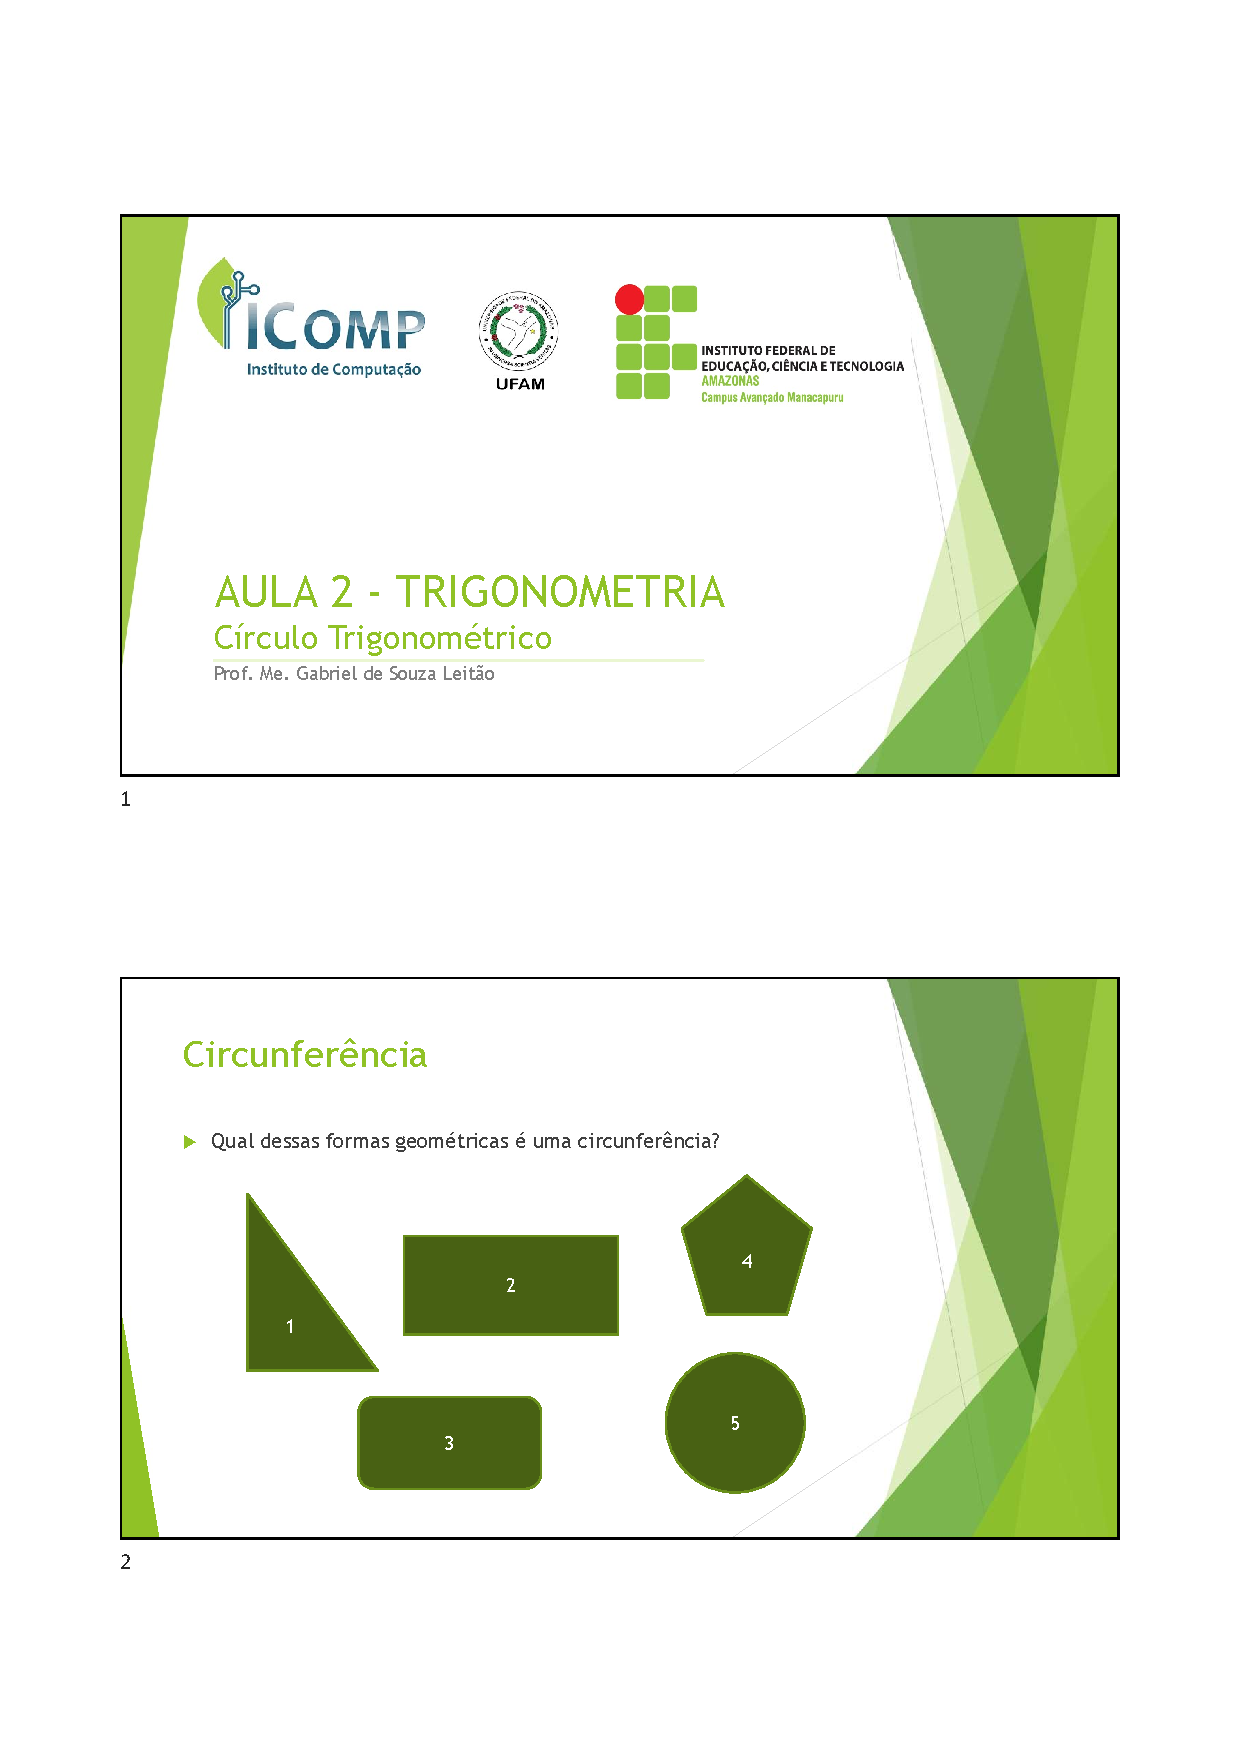
\includegraphics[width=\textwidth]{chapters/appendixLesson/Aula2.pdf}
%\end{figure}
%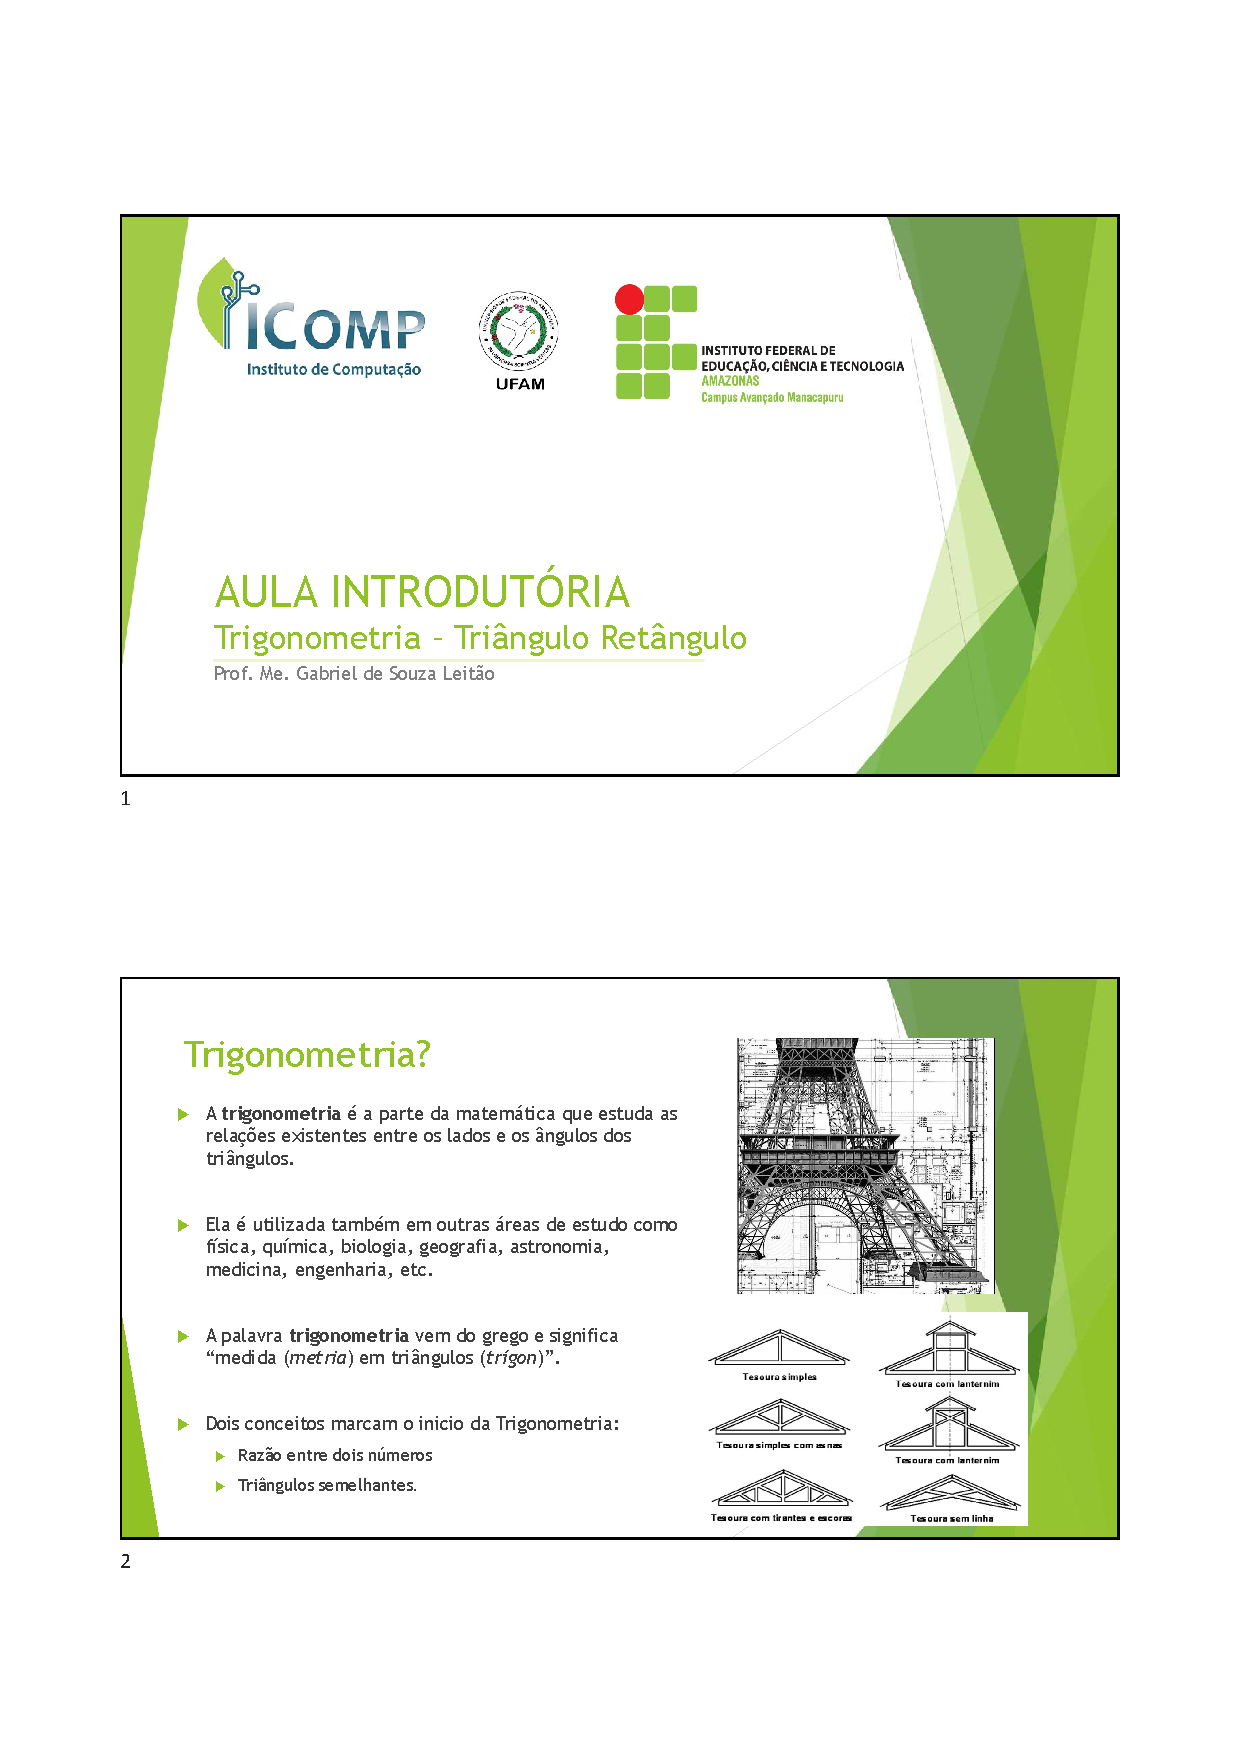
\includepdf[pages=-,offset=75 -75,pagecommand=\thispagestyle{plain}] {chapters/appendixLesson/Aula1Base20220611.pdf}
%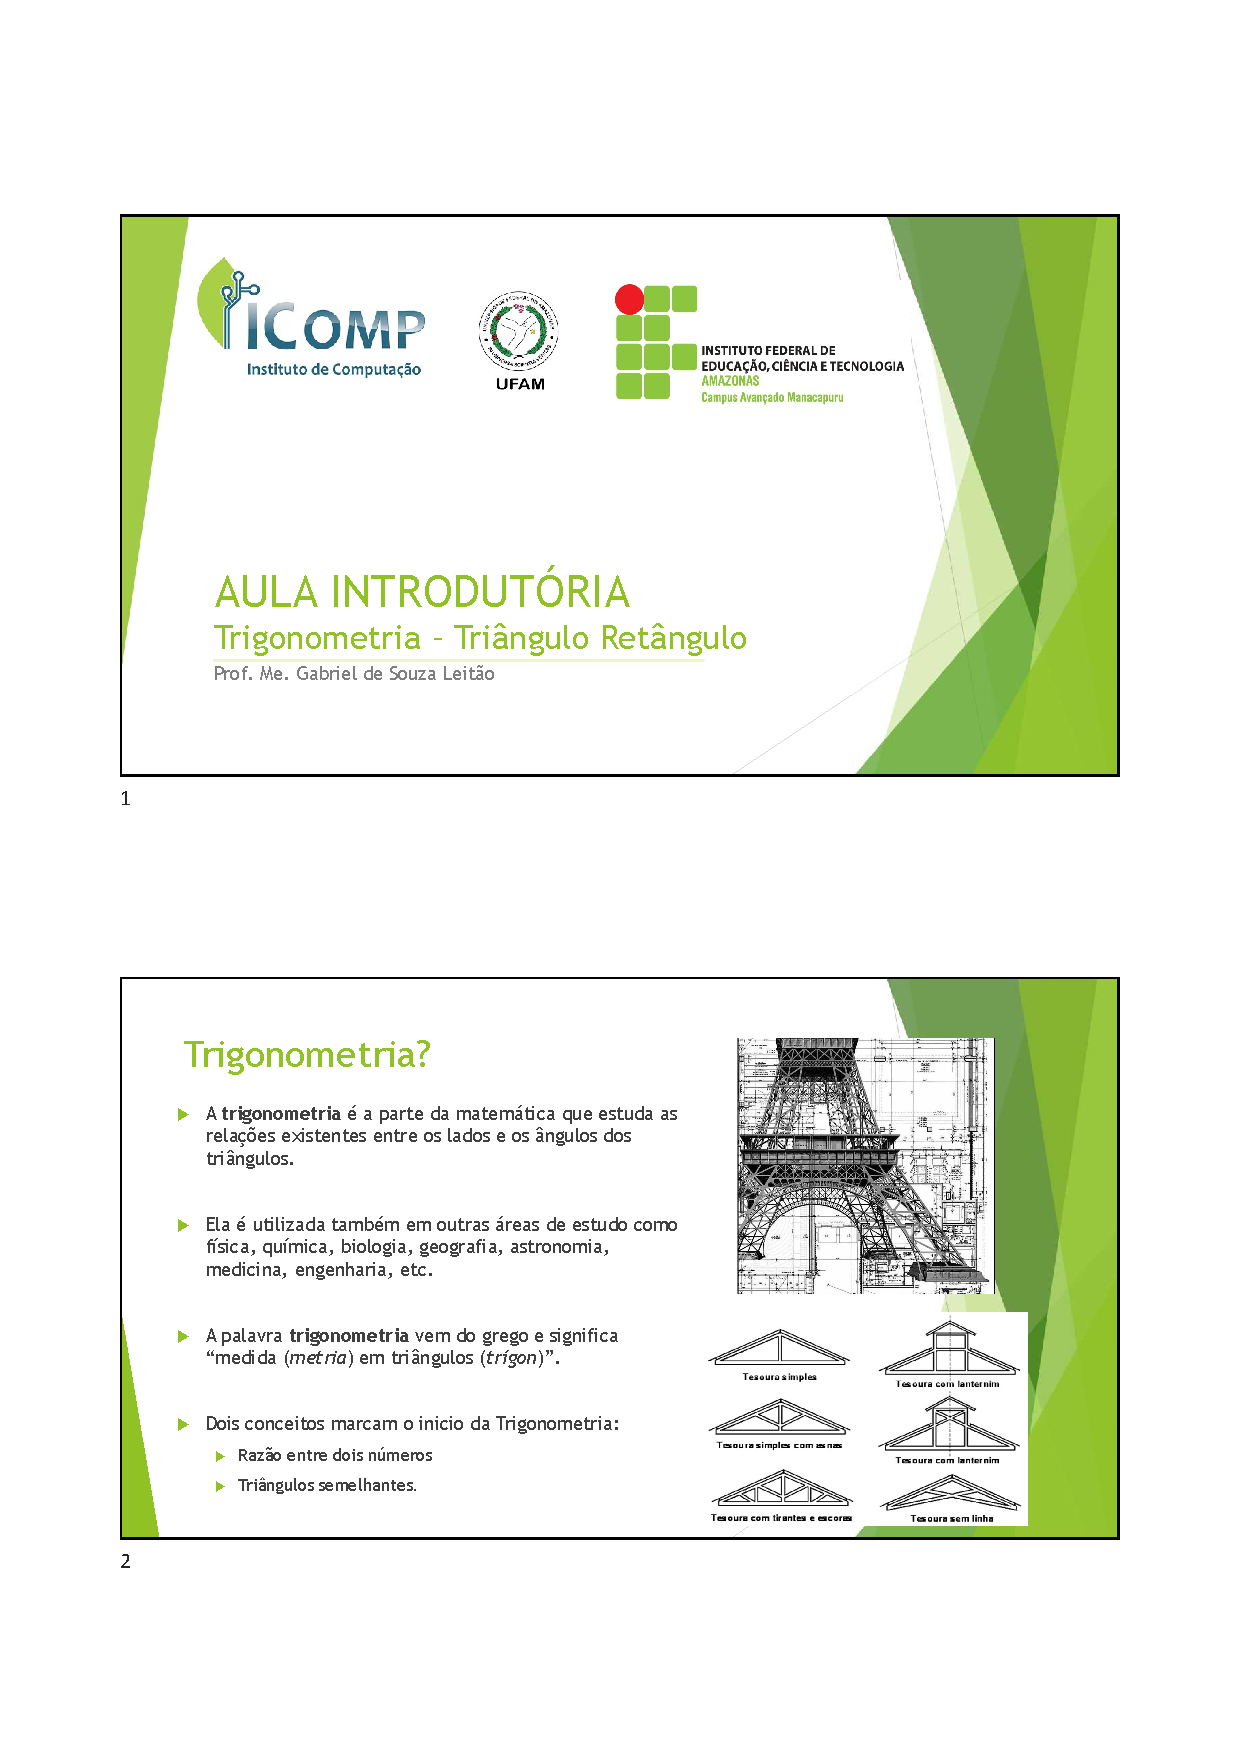
\includepdf[pages=-,pagecommand={},width=\textwidth]{chapters/appendixLesson/Aula1Base20220611.pdf}

%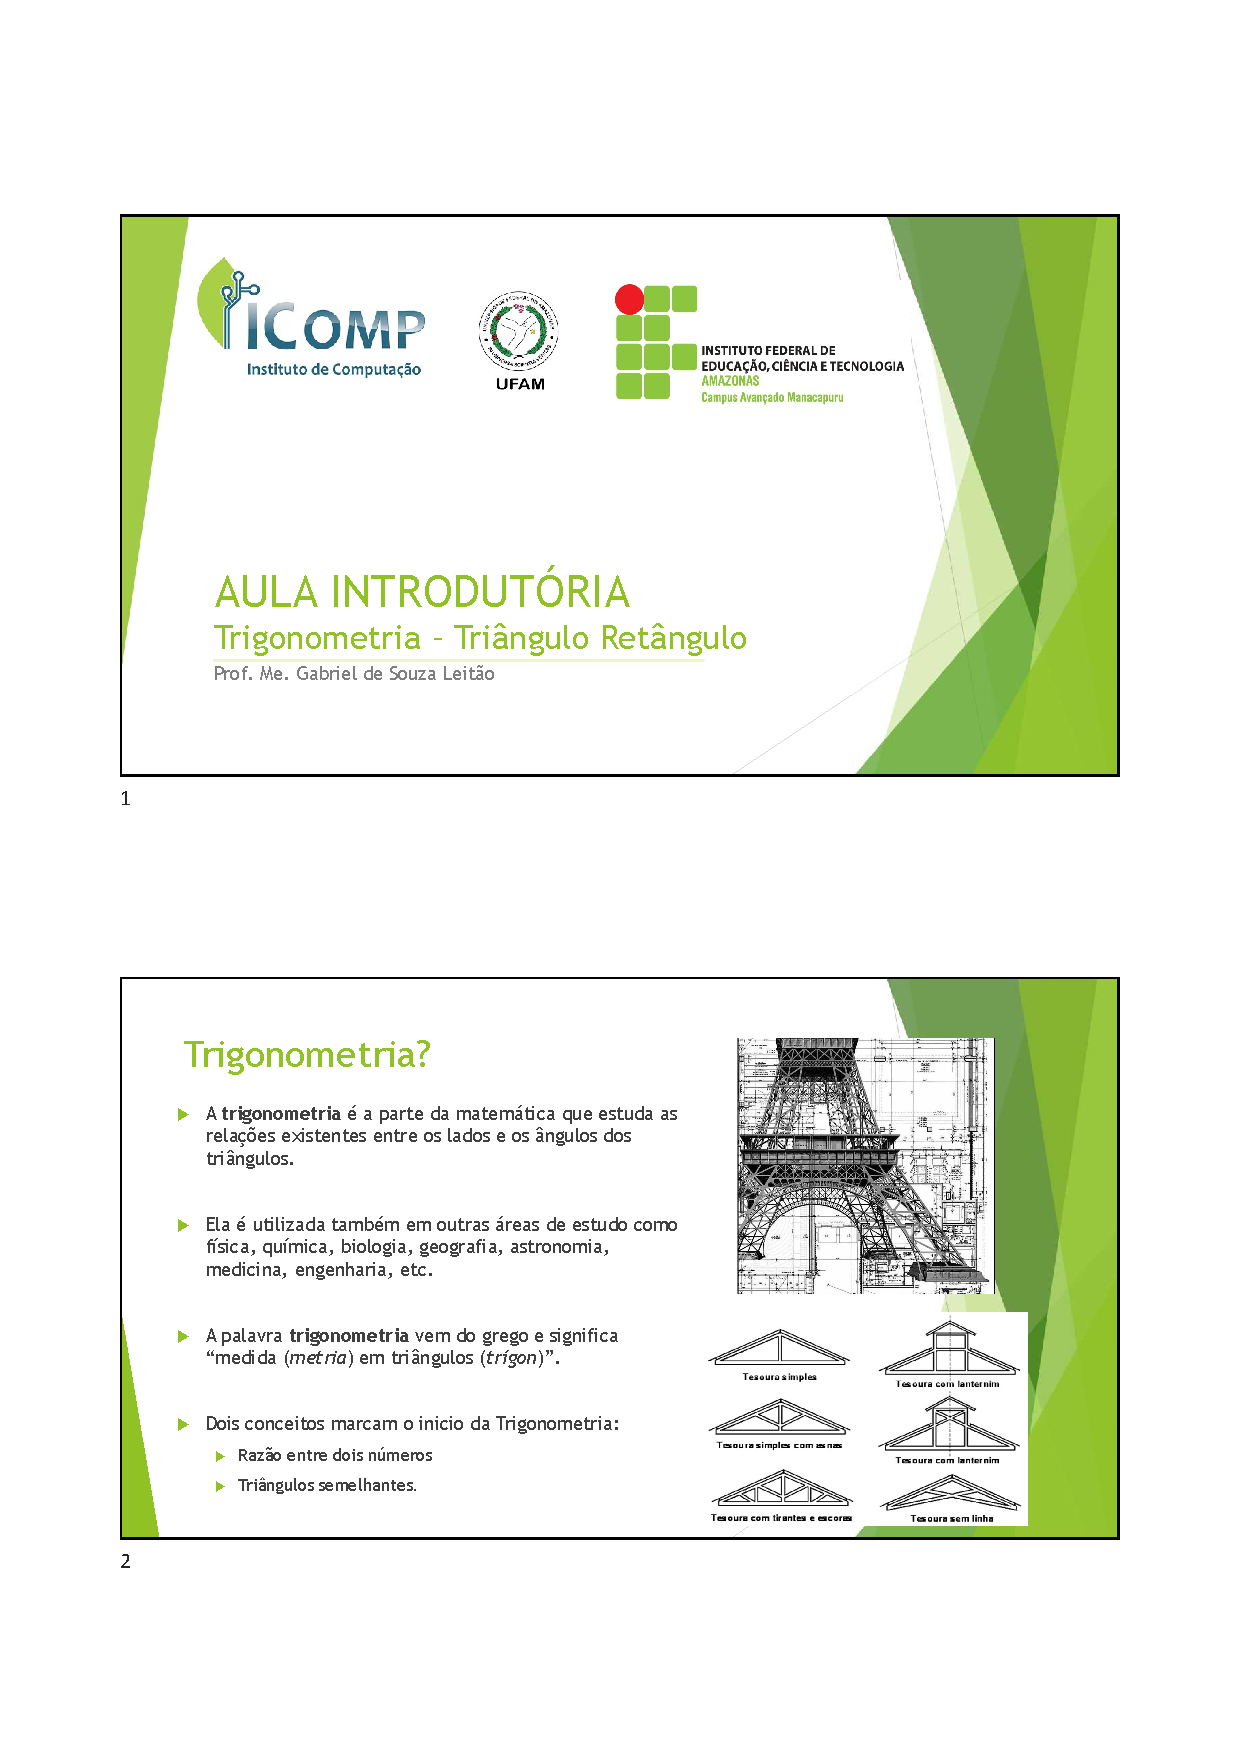
\includegraphics[scale=0.7,page=1]{chapters/appendixLesson/Aula1Base20220611.pdf}
\includegraphics[width=\textwidth,page=2]{chapters/appendixLesson/Aula2.pdf}
\includegraphics[width=\textwidth,page=3]{chapters/appendixLesson/Aula2.pdf}
\includegraphics[width=\textwidth,page=4]{chapters/appendixLesson/Aula2.pdf}
\includegraphics[width=\textwidth,page=5]{chapters/appendixLesson/Aula2.pdf}
\includegraphics[width=\textwidth,page=6]{chapters/appendixLesson/Aula2.pdf}
\includegraphics[width=\textwidth,page=7]{chapters/appendixLesson/Aula2.pdf}
\includegraphics[width=\textwidth,page=8]{chapters/appendixLesson/Aula2.pdf}
\includegraphics[width=\textwidth,page=9]{chapters/appendixLesson/Aula2.pdf}
\includegraphics[width=\textwidth,page=10]{chapters/appendixLesson/Aula2.pdf}
\includegraphics[width=\textwidth,page=11]{chapters/appendixLesson/Aula2.pdf}
\includegraphics[width=\textwidth,page=12]{chapters/appendixLesson/Aula2.pdf}
\includegraphics[width=\textwidth,page=13]{chapters/appendixLesson/Aula2.pdf}
\includegraphics[width=\textwidth,page=14]{chapters/appendixLesson/Aula2.pdf}
\includegraphics[width=\textwidth,page=15]{chapters/appendixLesson/Aula2.pdf}
\includegraphics[width=\textwidth,page=16]{chapters/appendixLesson/Aula2.pdf}
\includegraphics[width=\textwidth,page=17]{chapters/appendixLesson/Aula2.pdf}

\section{Atividade 2: Exercício de Fixação}\label{section:atividade2_fixação}

\begin{center}
	\textbf{\Large Exercício de Fixação}
\end{center}

\textbf{1 – Complete a tabela abaixo, indicando os intervalos de variação, em graus e em radianos, de cada quadrante:}

\begin{table}[htb]
	\centering
	\begin{tabular}{|l|l|l|}
		\hline
		\multicolumn{1}{|c|}{\textbf{Quadrante}} & \multicolumn{1}{c|}{\textbf{Intervalo em graus}} & \multicolumn{1}{c|}{\textbf{Intervalo em radianos}} \\ \hline
		\textbf{1º Quadrante} &  &  \\ \hline
		\textbf{2º Quadrante} &  &  \\ \hline
		\textbf{3º Quadrante} &  &  \\ \hline
		\textbf{4º Quadrante} &  &  \\ \hline
	\end{tabular}
\end{table}


\textbf{2 – Com o auxílio de um transferidor, marque no círculo trigonométrico os pontos que correspondem aos ângulos:}

$15^\circ, 75^\circ, 30^\circ, 60^\circ, \pi/4, 120^\circ, 150^\circ, \frac{3\pi}{4}, \frac{7\pi}{6}, 240^\circ, \frac{5\pi}{3}, 330^\circ, 420^\circ, 480^\circ, 540^\circ, 600^\circ, 750^\circ, 780^\circ,\\ \frac{-\pi}{3}, -135^\circ, -225^\circ$


\begin{figure}[htb]
	\centering
	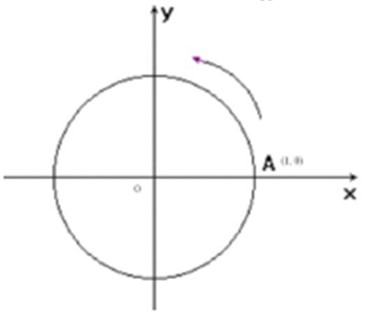
\includegraphics{chapters/appendixLesson/Q2.jpg}
\end{figure}

\textbf{3 – Cada sentença apresenta resultados para o seno de um ângulo desconhecido x. Usando o círculo trigonométrico, encontre valores de x, que satisfaçam as sentenças:}

\begin{table}[htb]
	\begin{tabular}{ll}
	 	a) sen x = 0,77 & c) sen x = 0,50 \\
		b) sen x = -0,34 & d) sen x = 0,80
	\end{tabular}
\end{table}

\textbf{4 – Cada sentença apresenta resultados para o cosseno de um ângulo desconhecido x. Usando o círculo trigonométrico, encontre valores de x, que satisfaçam as sentenças:}

\begin{table}[htb]
	\begin{tabular}{ll}
		a) cos x = 0,77 & c) cos x = 0,50 \\
		b) cos x = -0,34 & d) cos x = 0,80
	\end{tabular}
\end{table}

\begin{figure}[htb]
	\centering
	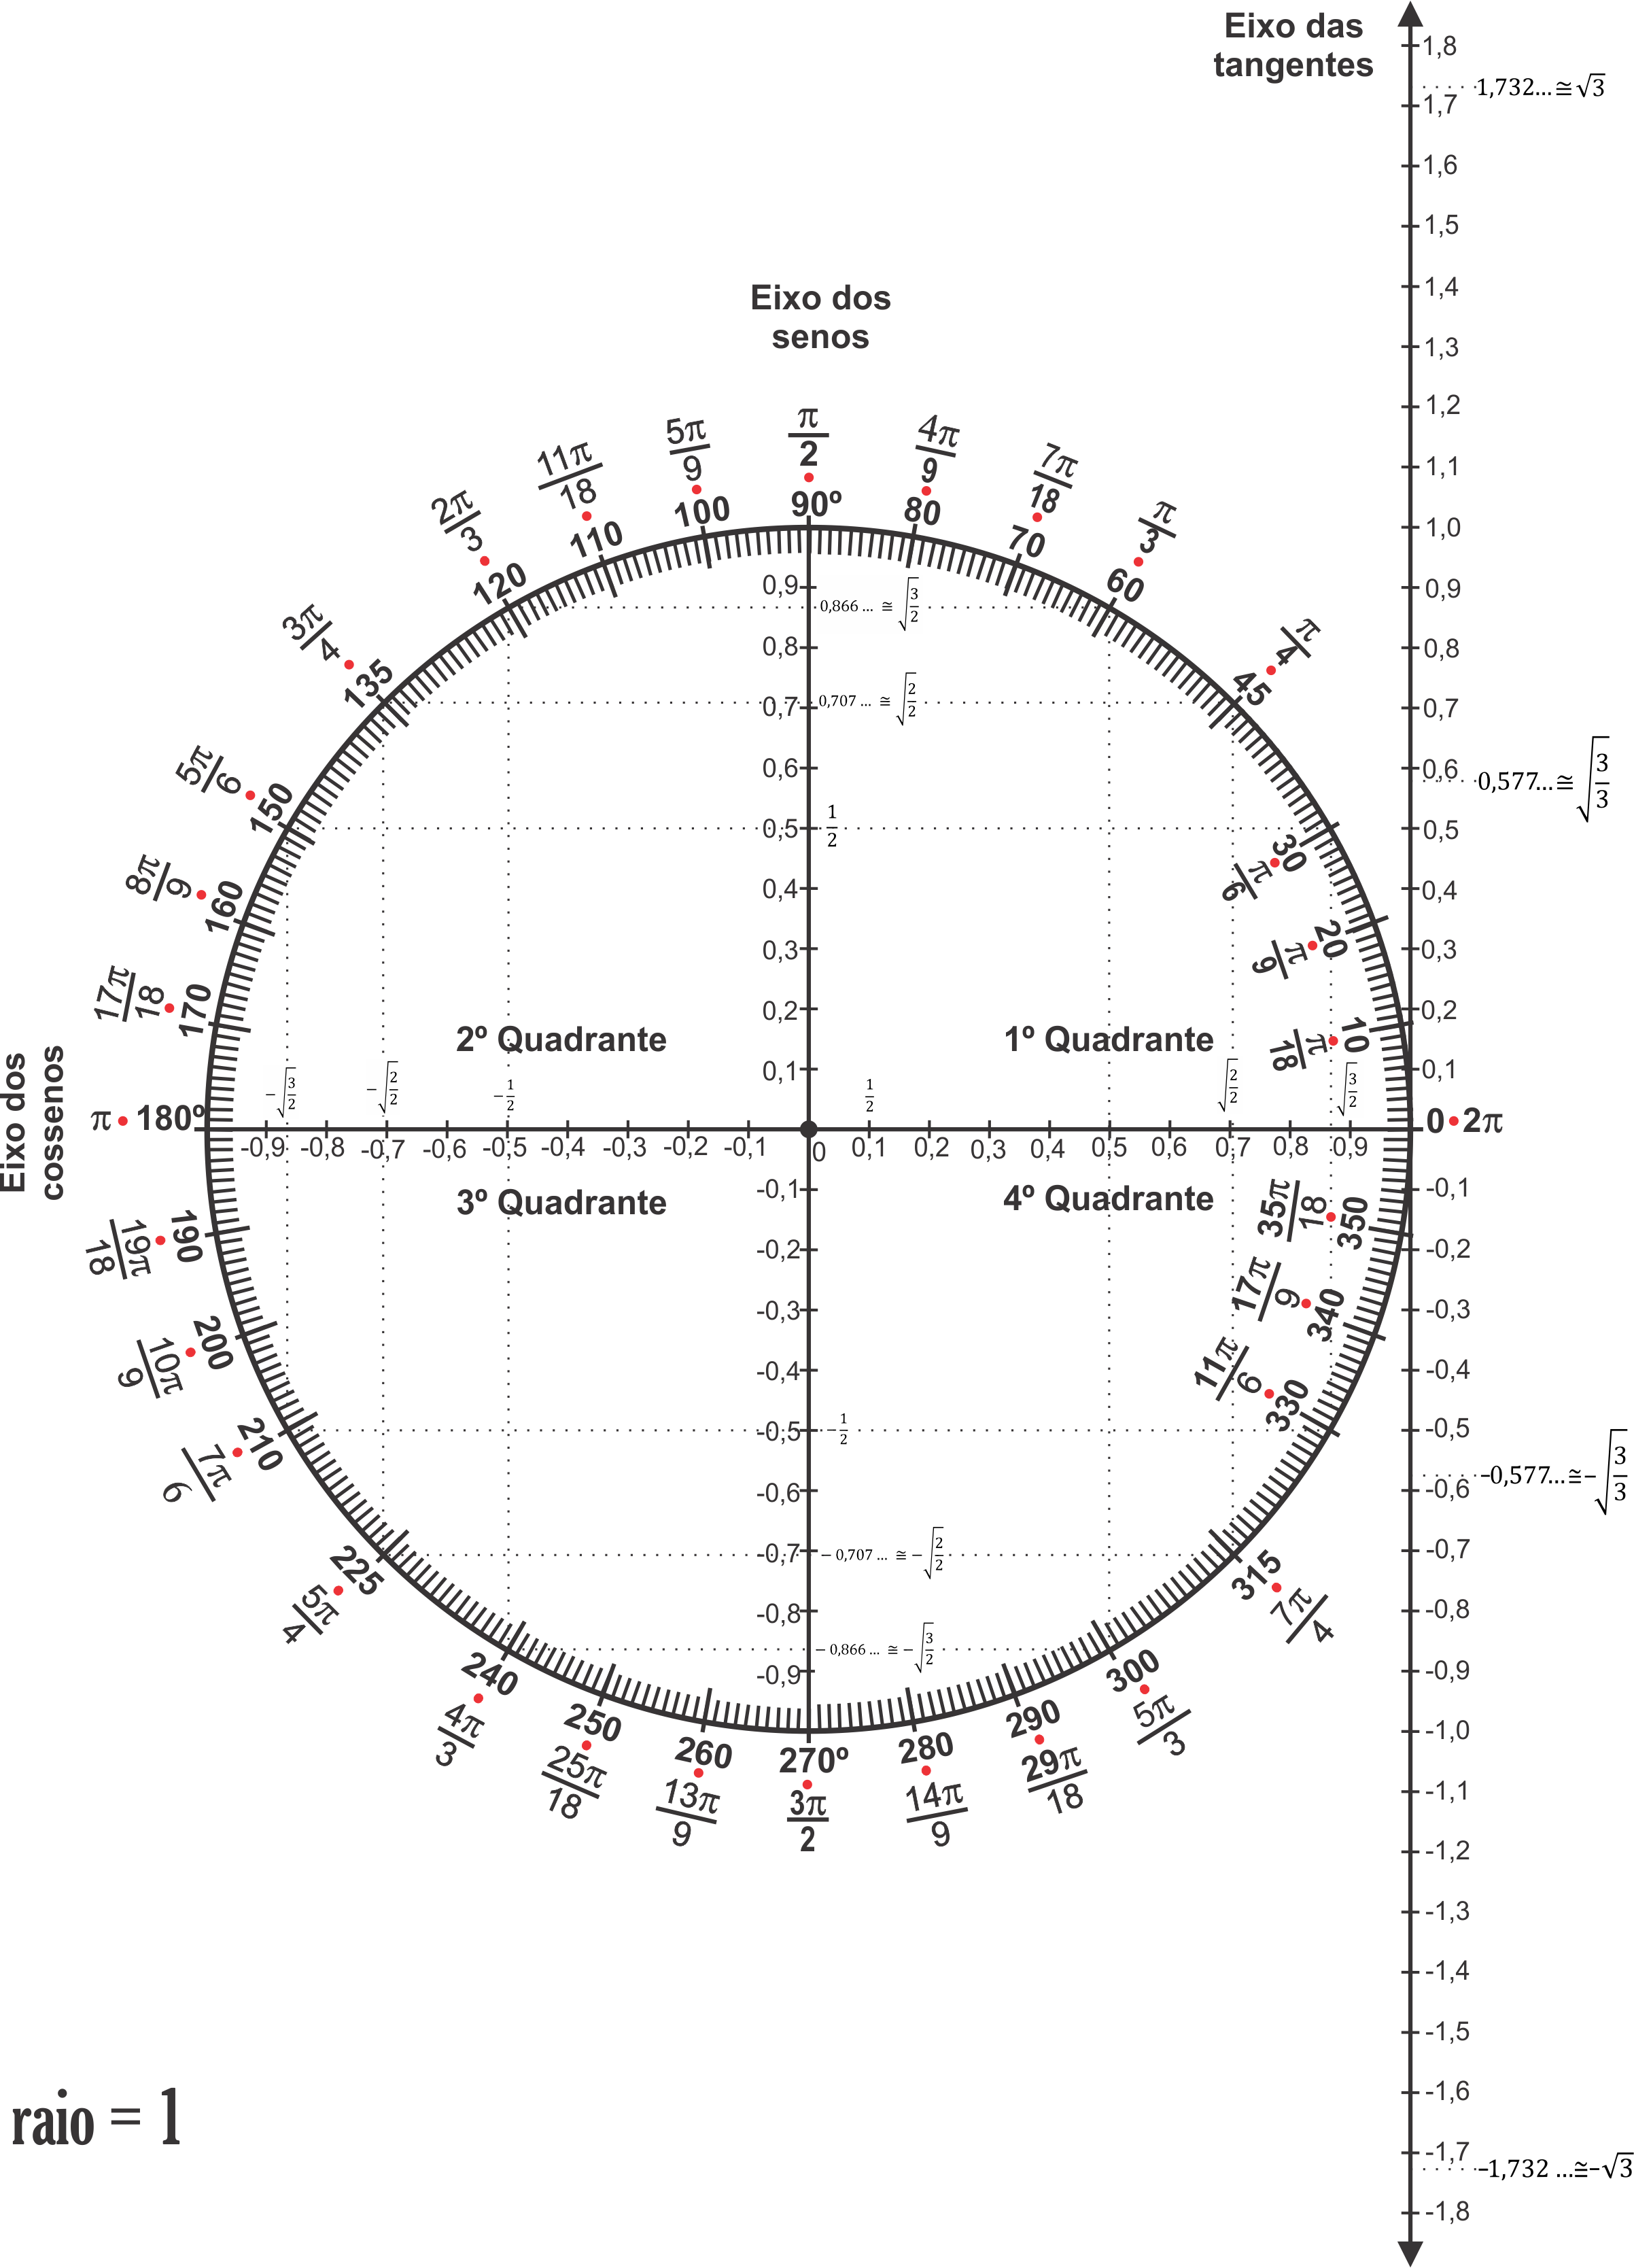
\includegraphics[width=\linewidth]{chapters/appendixLesson/circulo_trigonometrico.png}
\end{figure}

%\textcolor{white}{texto a ser colorido}
%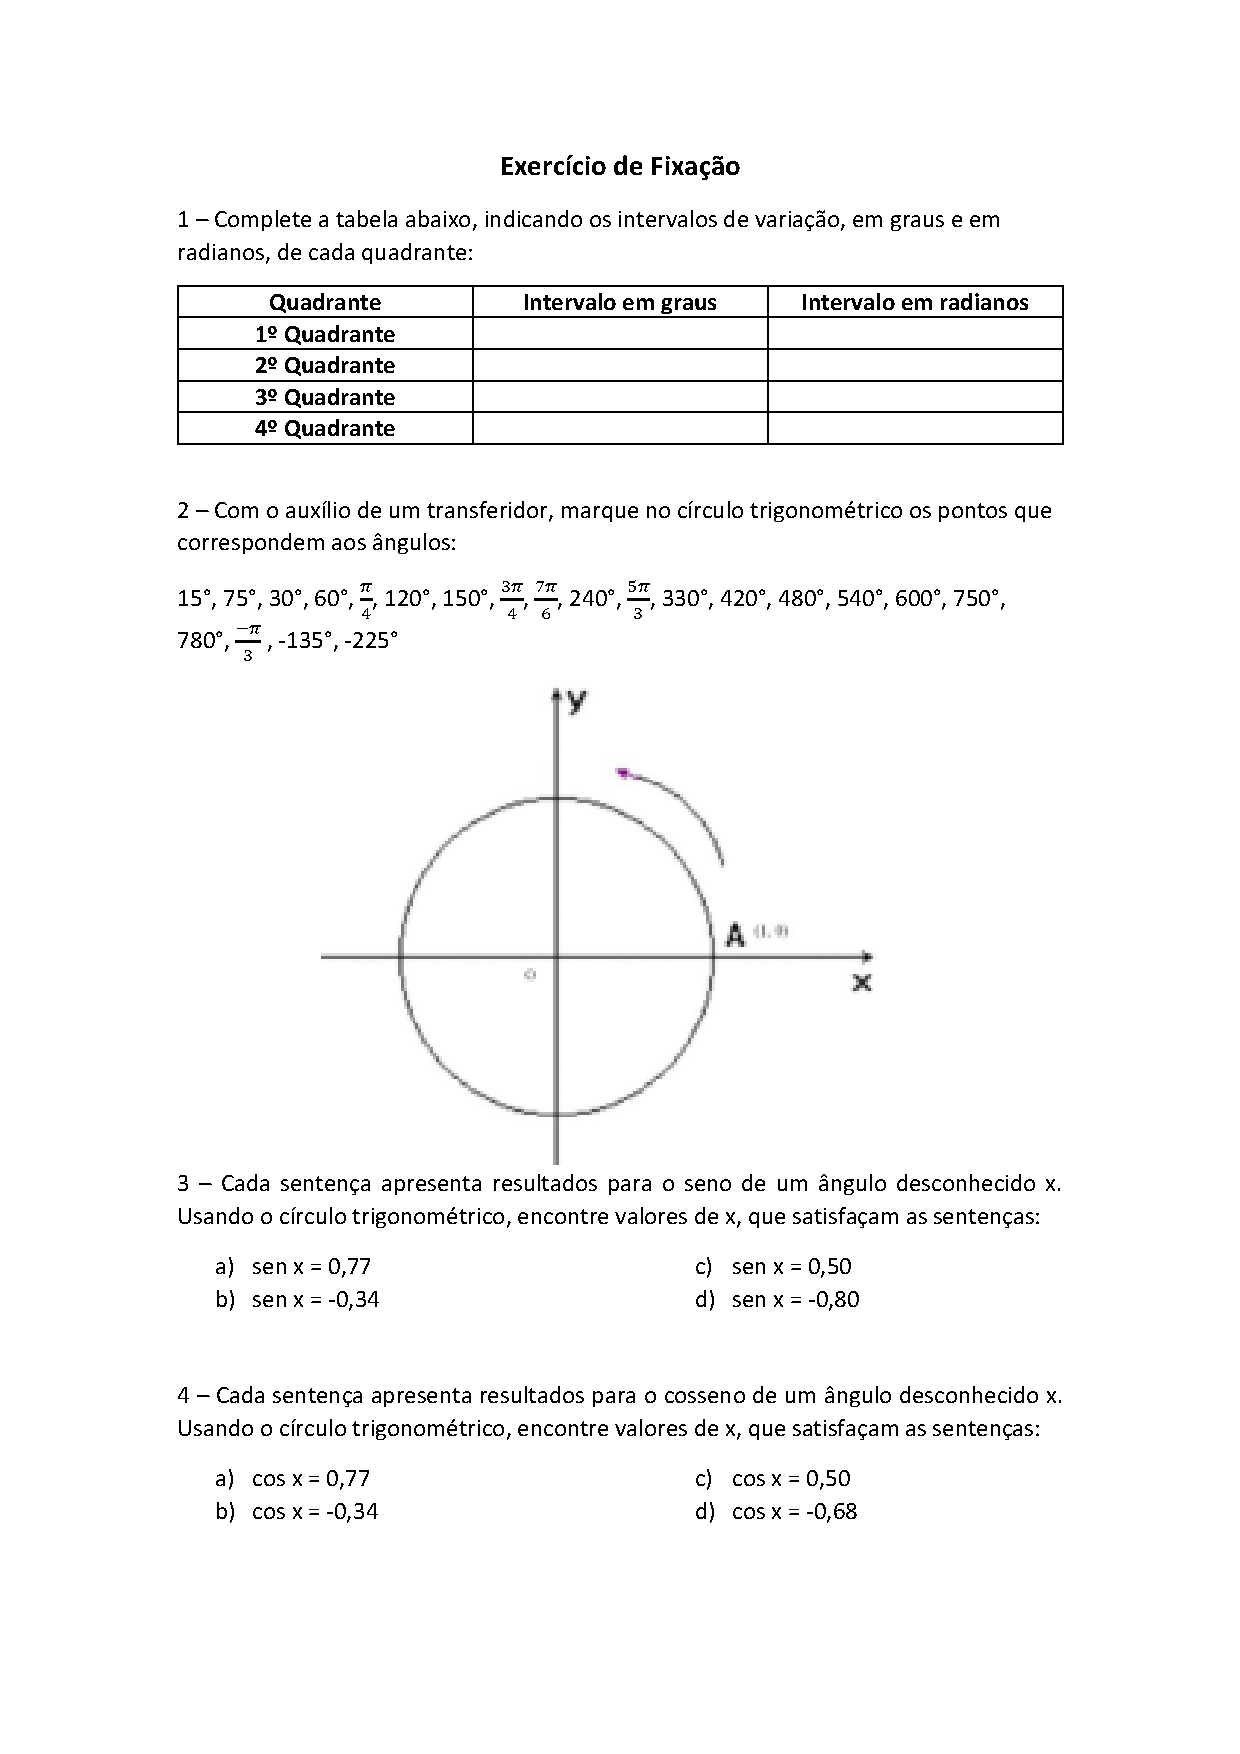
\includegraphics[width=1.1\textwidth]{chapters/appendixLesson/ExercícioFixação.pdf}
%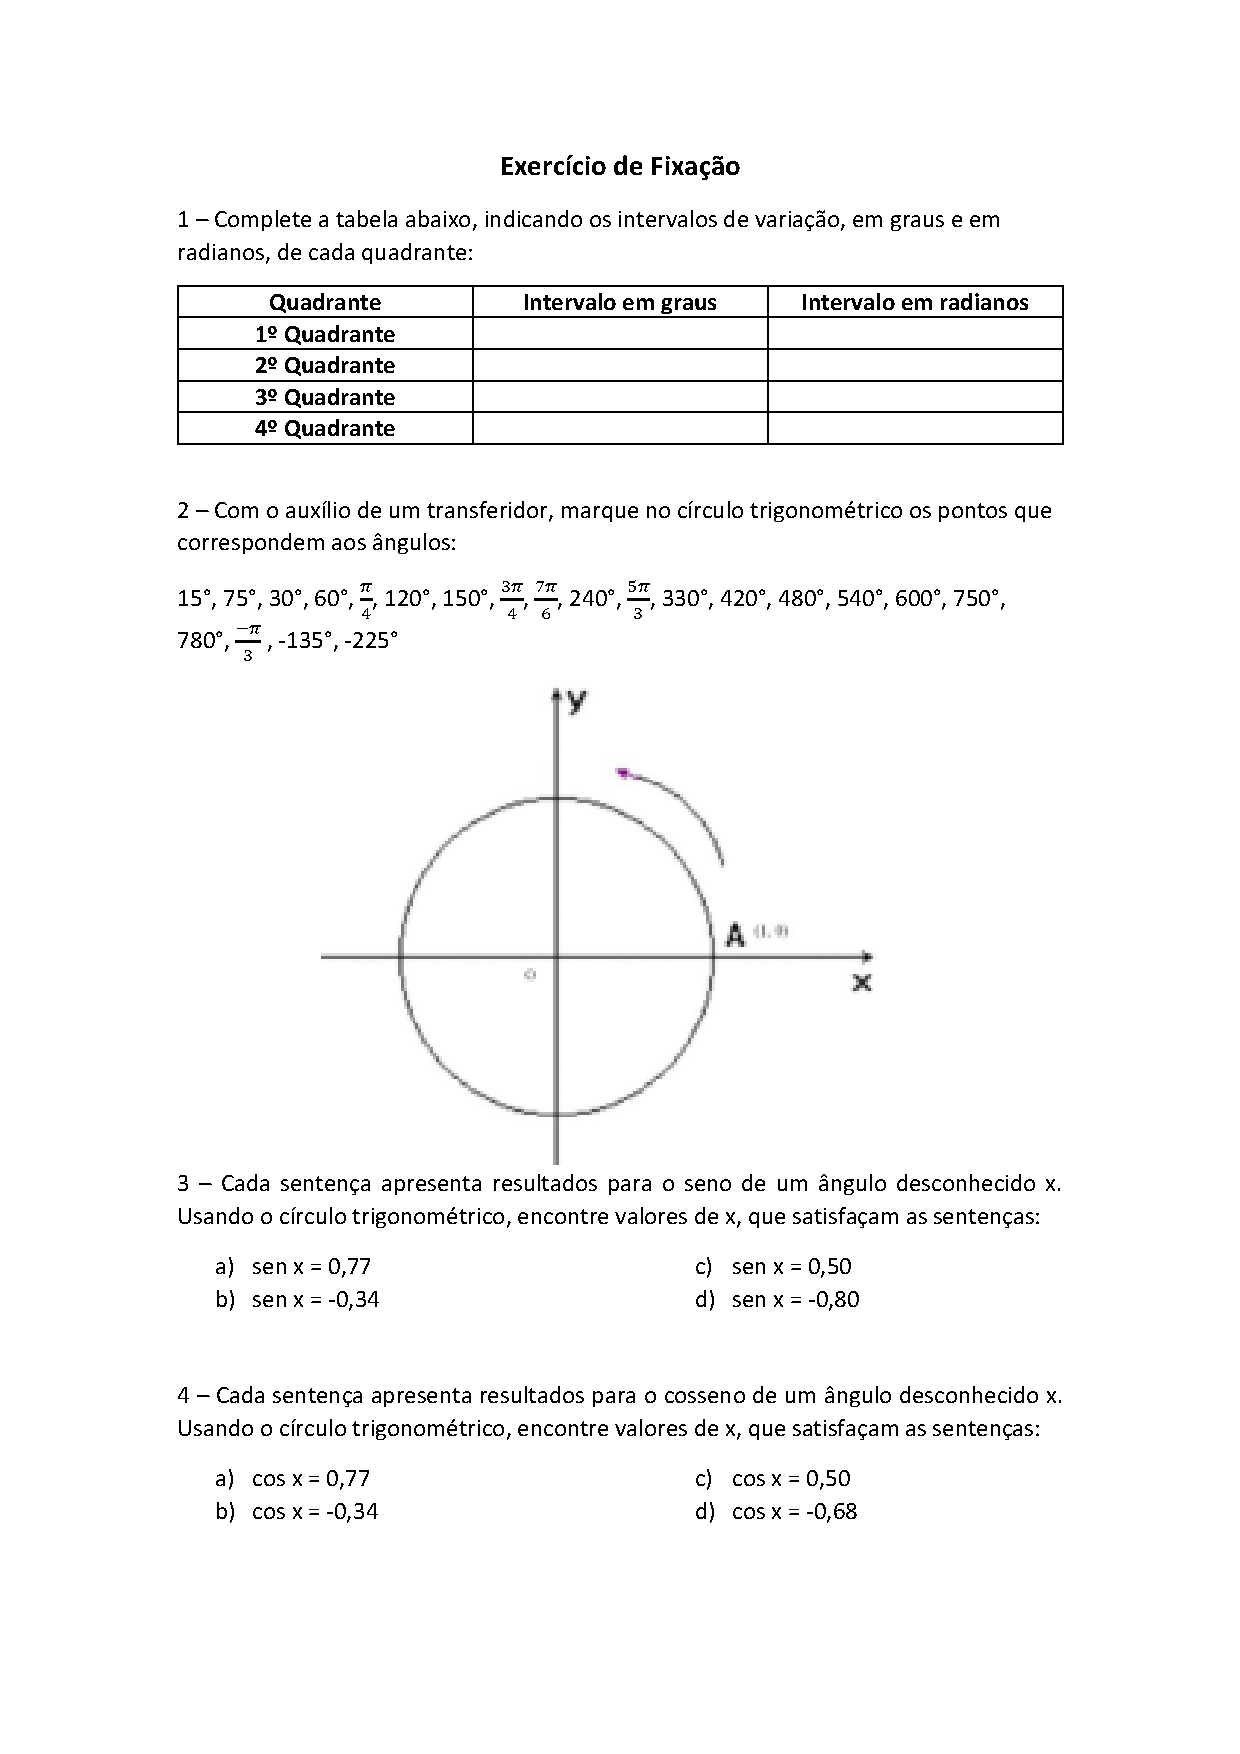
\includegraphics[width=\textwidth]{chapters/appendixLesson/ExercícioFixação.pdf}
%\includegraphics[width=\textwidth,page=2]{chapters/appendixLesson/ExercícioFixação.pdf}

\clearpage

\section{Atividade 3: Interfaces Físicas do Player Tangível}\label{section:atividade3_interfaces}

Esta seção apresenta as interfaces trocáveis do objeto tangível de modo que cada interface corresponde a um exercício distinto.

\subsection{Interface Física A01}\label{subsection:atividade3_A01}
\begin{figure}[htb]
	\centering
	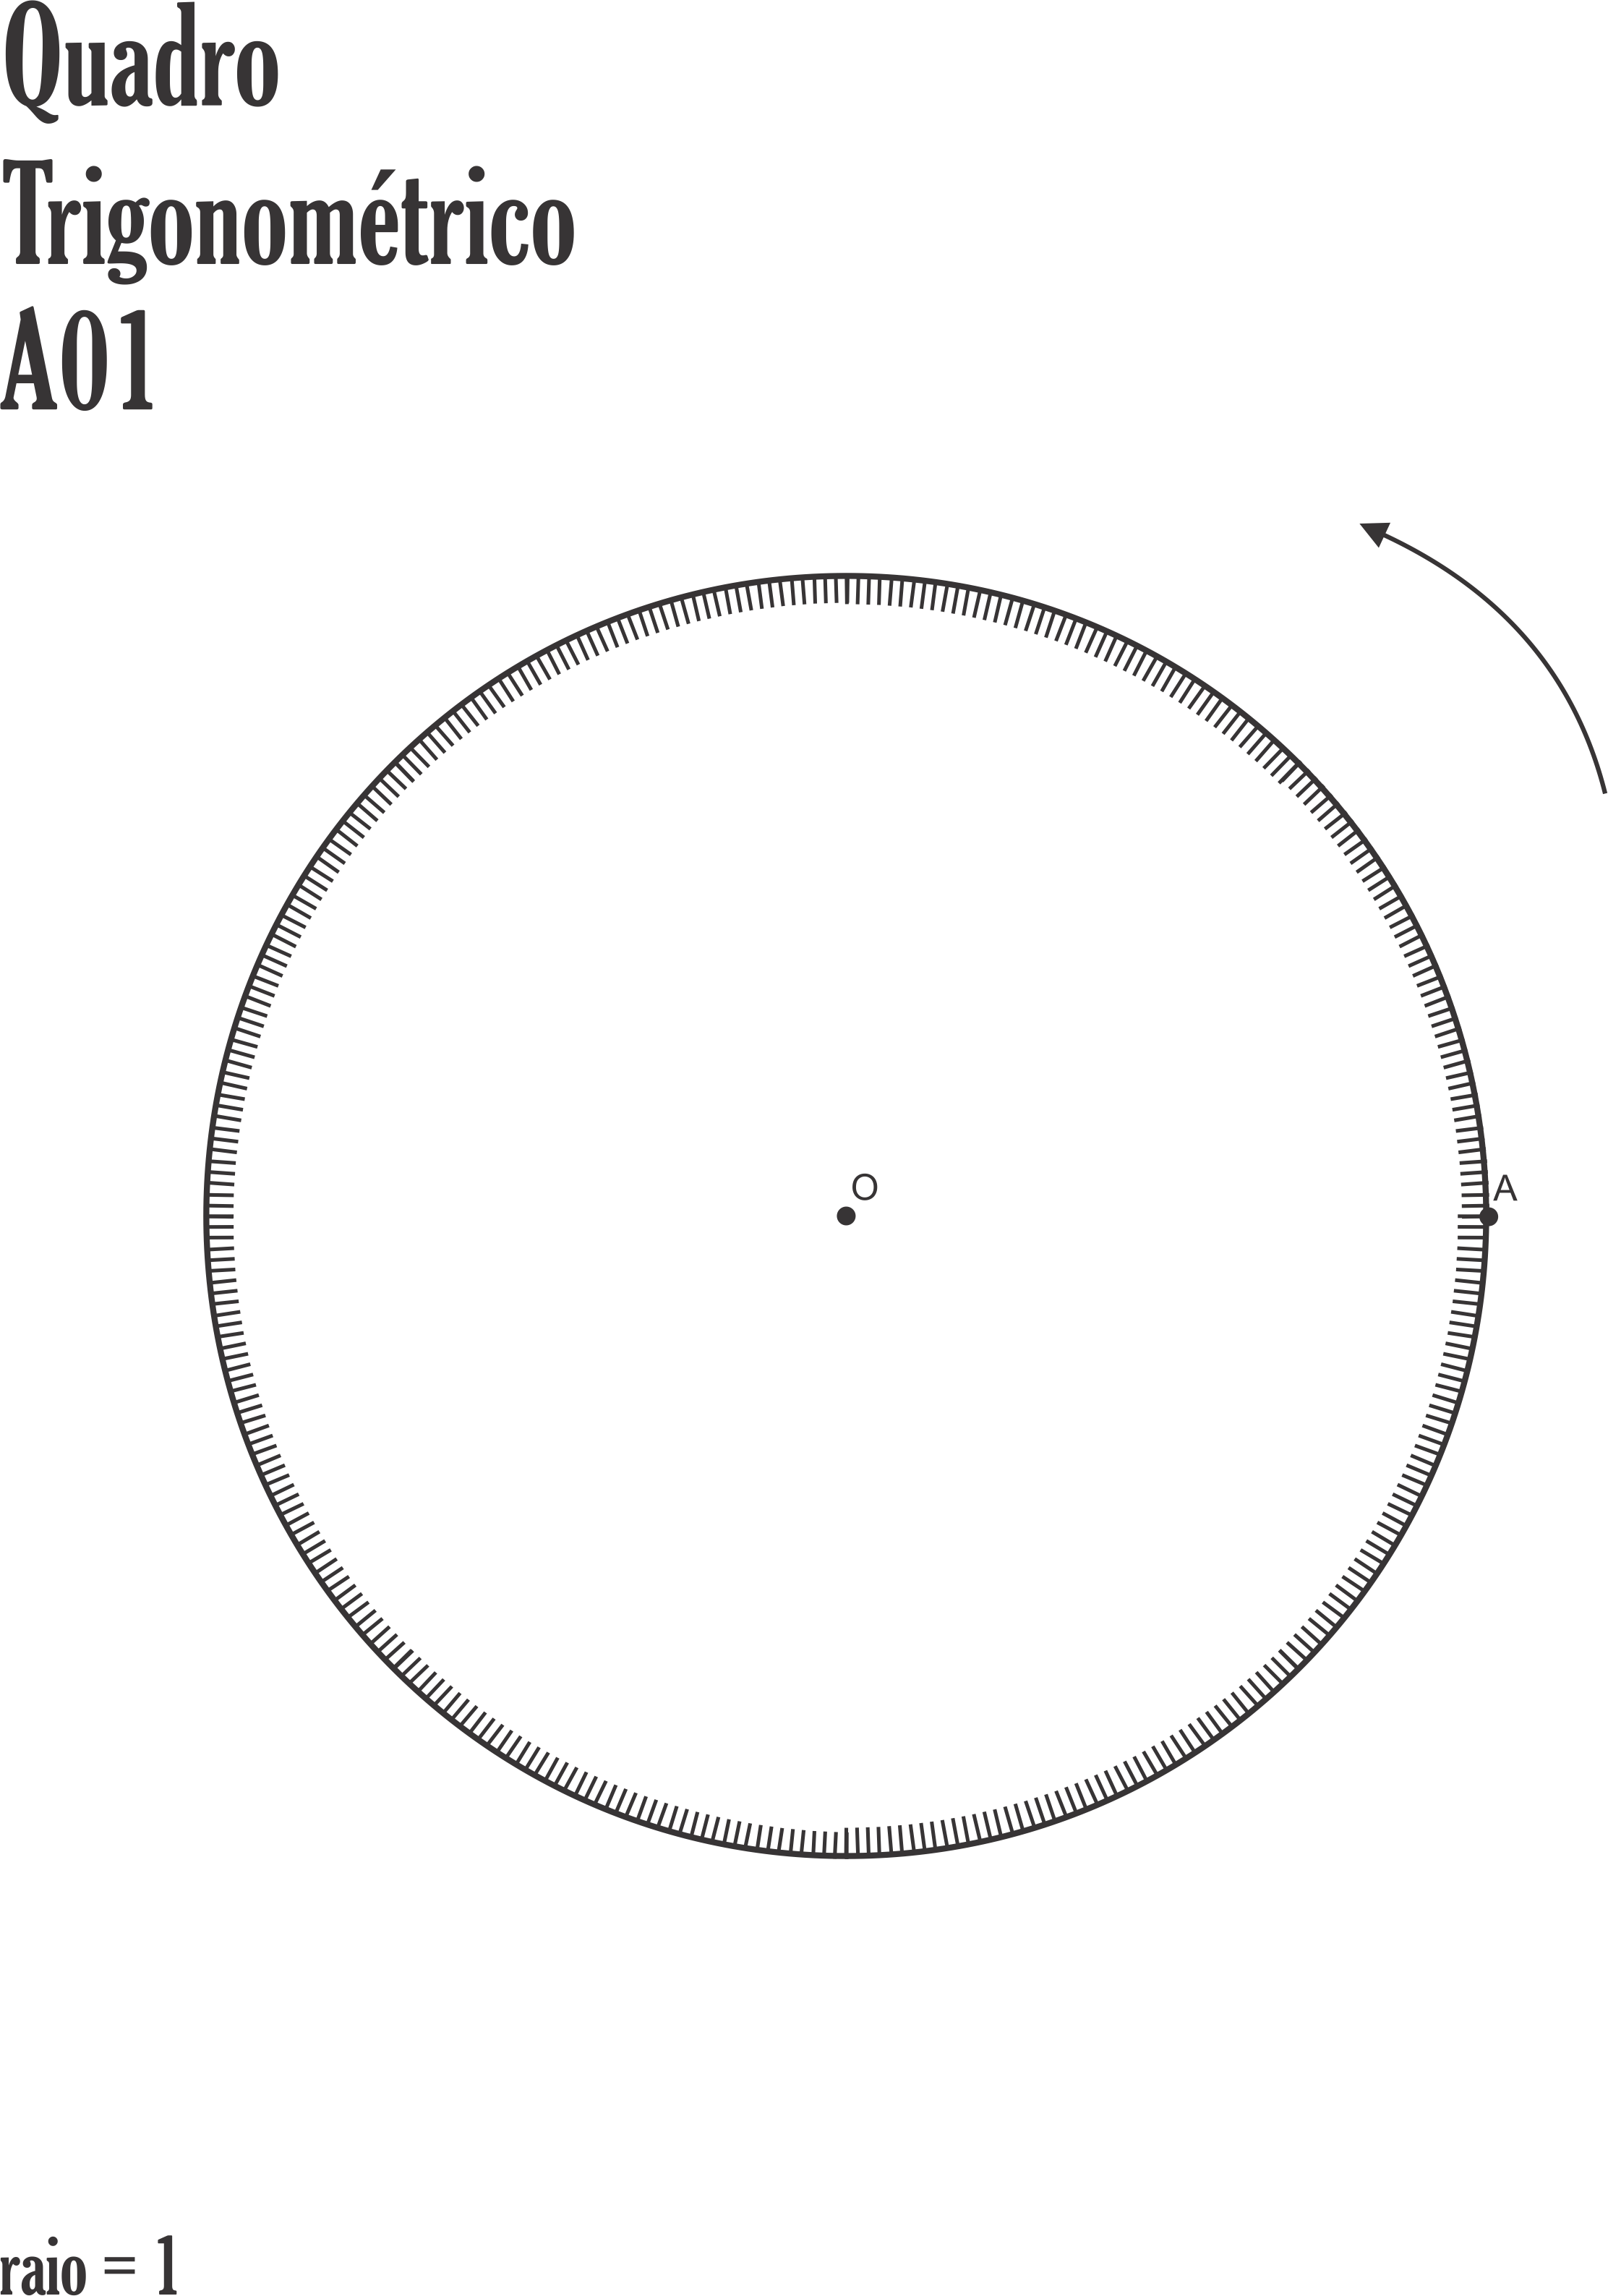
\includegraphics[width=0.9\linewidth]{chapters/appendixLesson/Interface_A01.png}
\end{figure}
\clearpage

\subsection{Interface Física A02}\label{subsection:atividade3_A02}
\begin{figure}[htb]
	\centering
	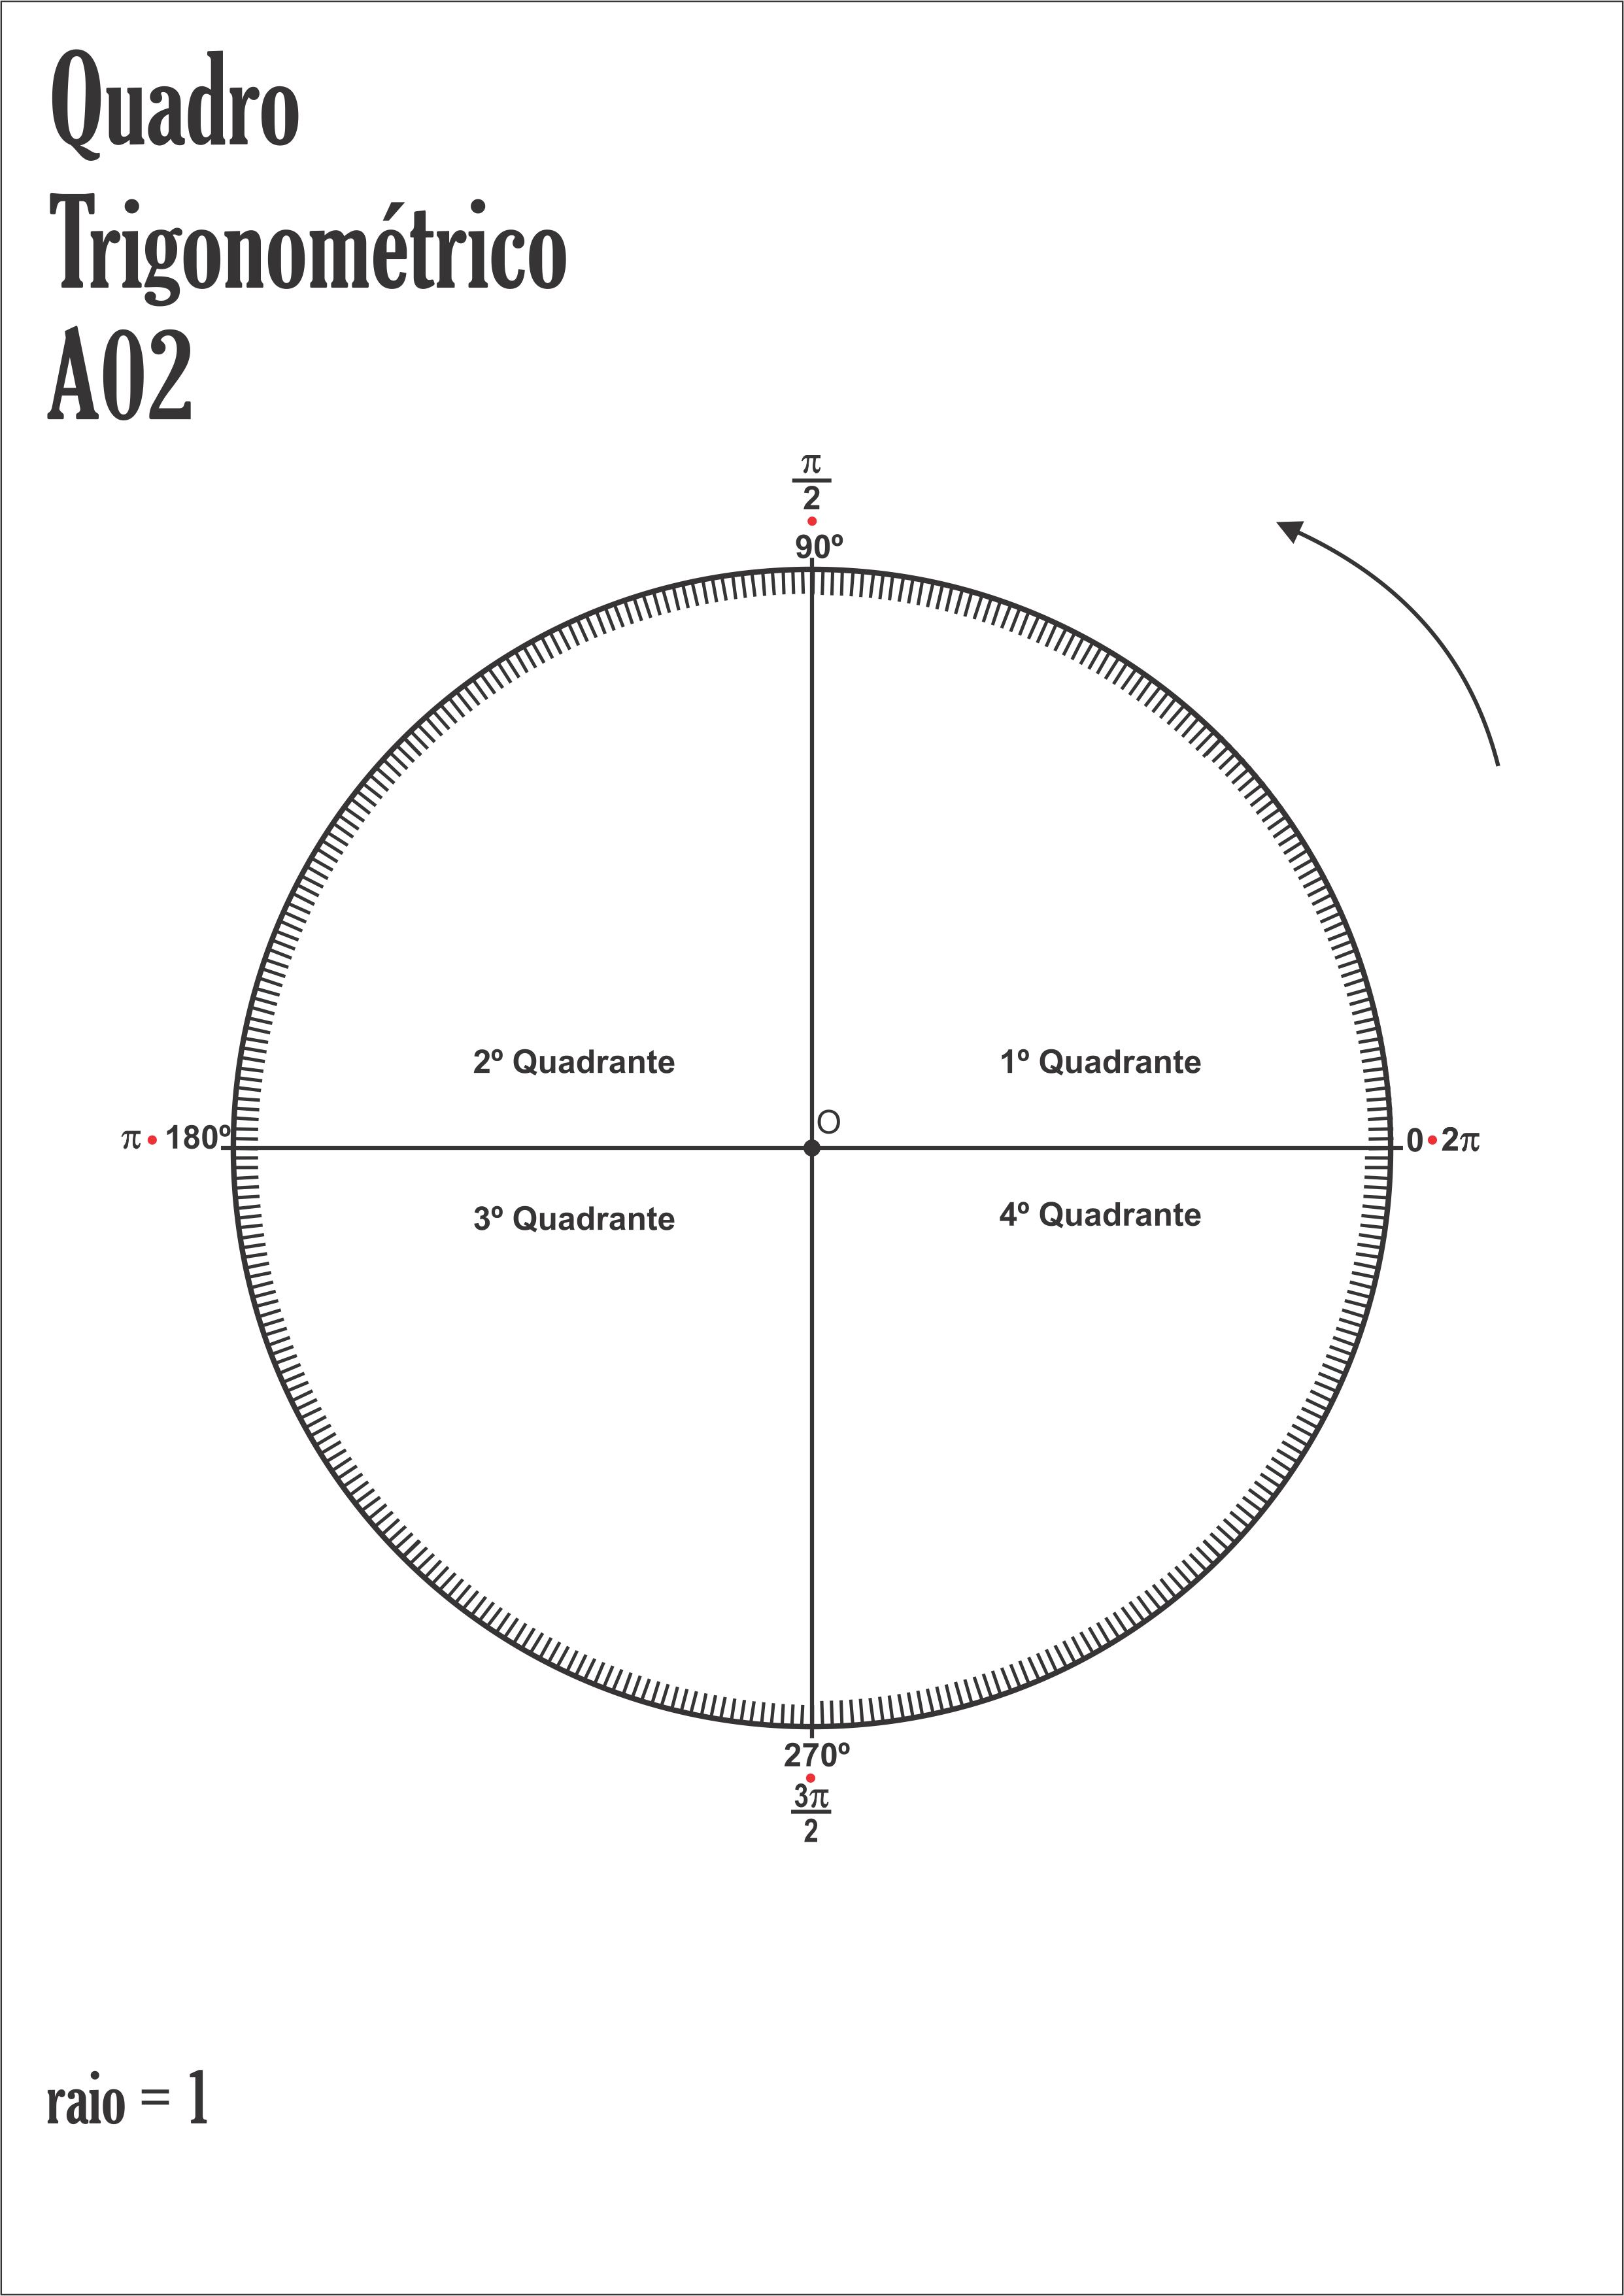
\includegraphics[width=0.9\linewidth]{chapters/appendixLesson/Interface_A02.png}
\end{figure}
\clearpage

\subsection{Interface Física A03}\label{subsection:atividade3_A03}
\begin{figure}[htb]
	\centering
	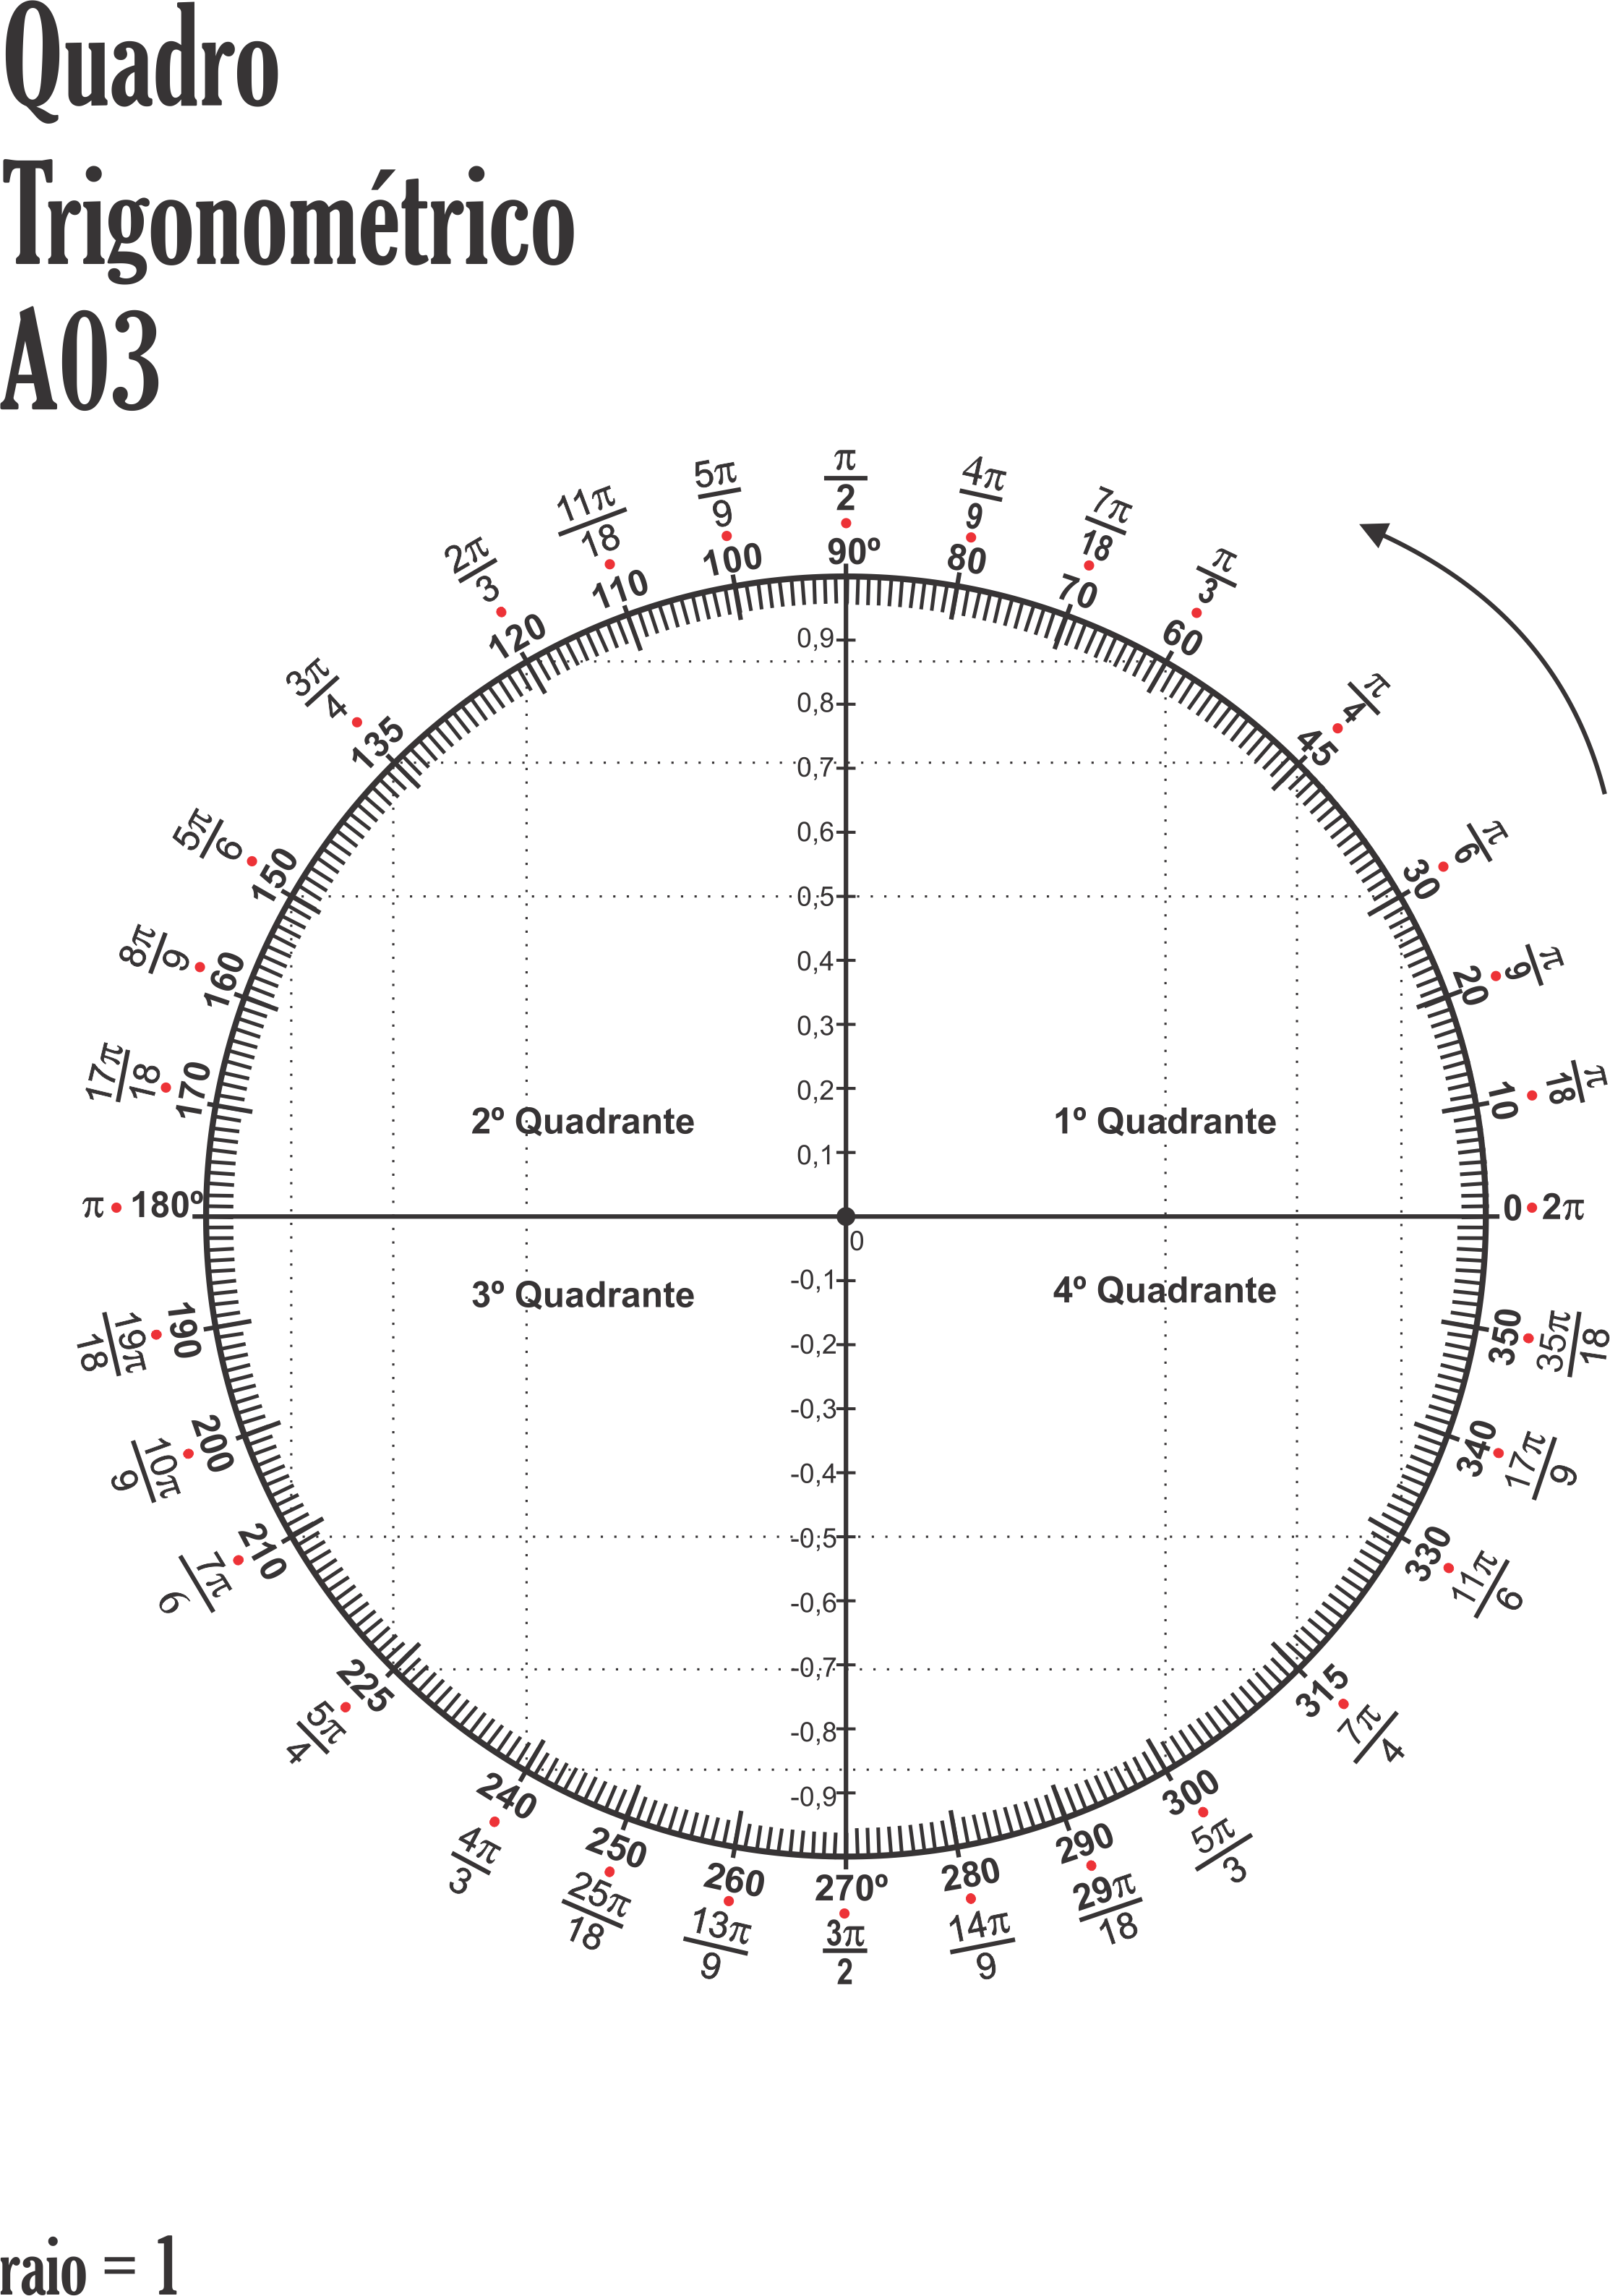
\includegraphics[width=0.9\linewidth]{chapters/appendixLesson/Interface_A03.png}
\end{figure}
\clearpage

\subsection{Interface Física A04}\label{subsection:atividade3_A04}
\begin{figure}[htb]
	\centering
	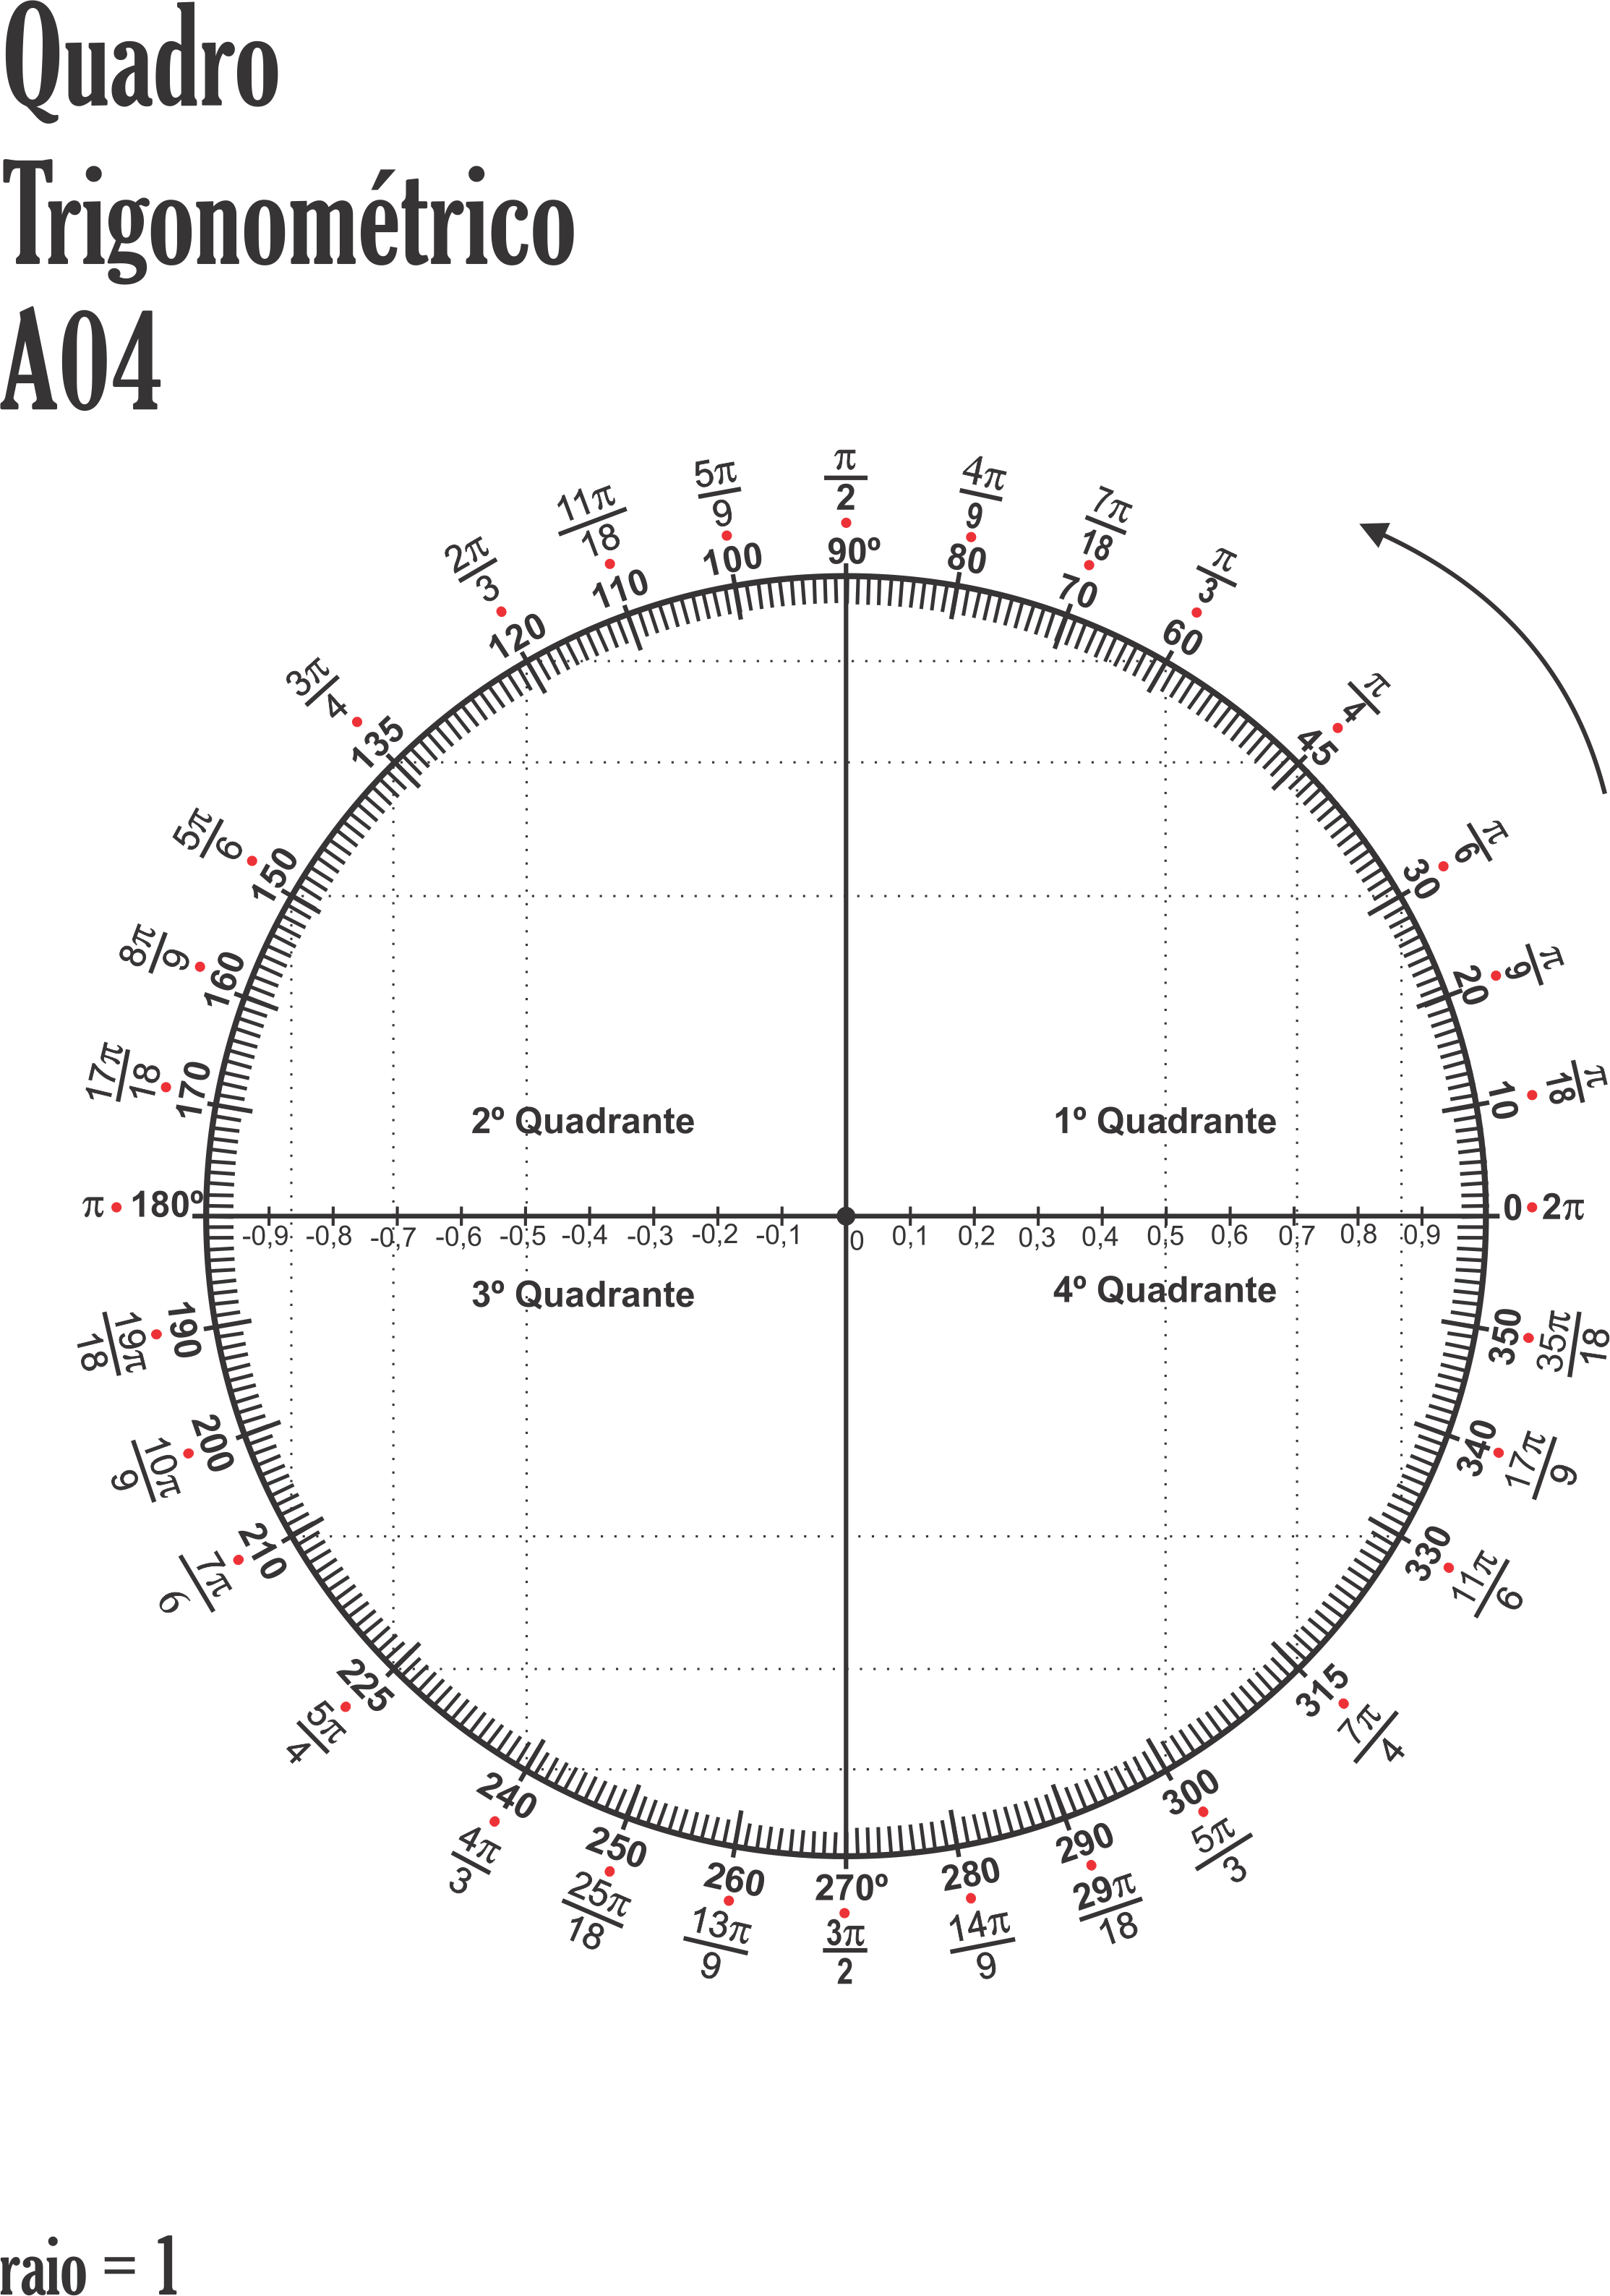
\includegraphics[width=0.9\linewidth]{chapters/appendixLesson/Interface_A04.png}
\end{figure}
\clearpage

\subsection{Interface Física A05}\label{subsection:atividade3_A05}
\begin{figure}[htb]
	\centering
	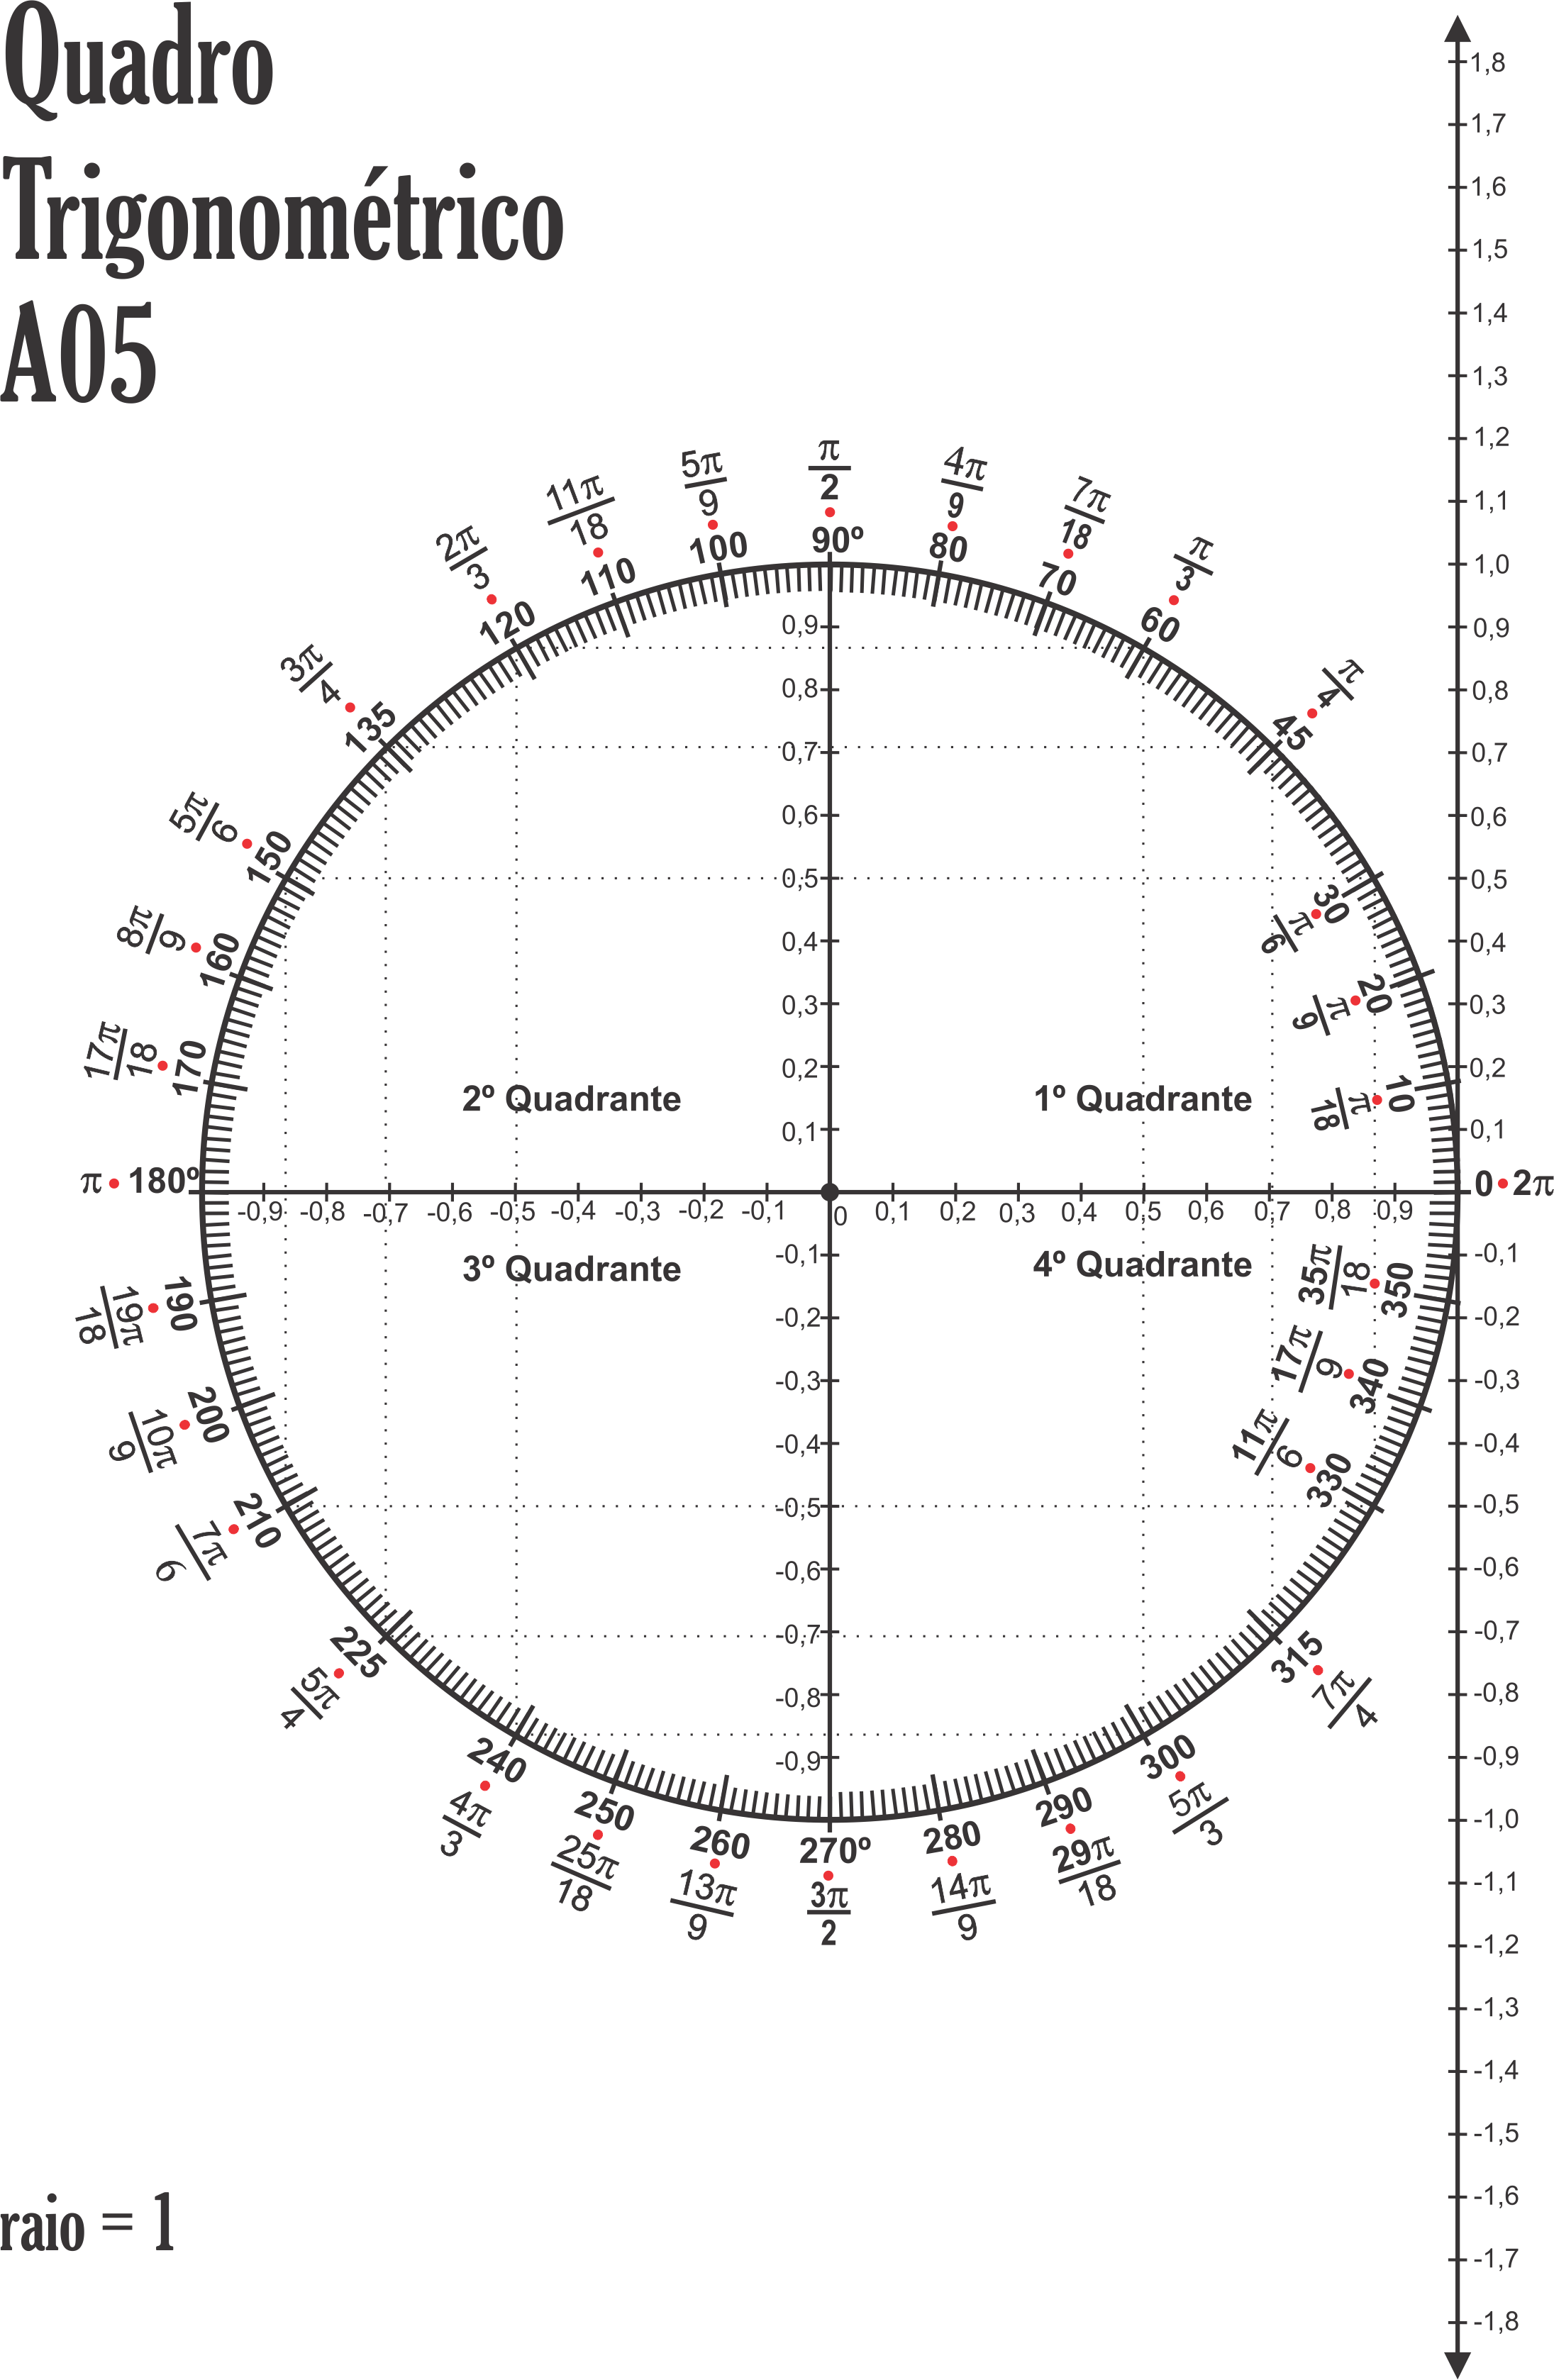
\includegraphics[width=0.9\linewidth]{chapters/appendixLesson/Interface_A05.png}
\end{figure}
\clearpage

\subsection{Interface Física A06}\label{subsection:atividade3_A06}
\begin{figure}[htb]
	\centering
	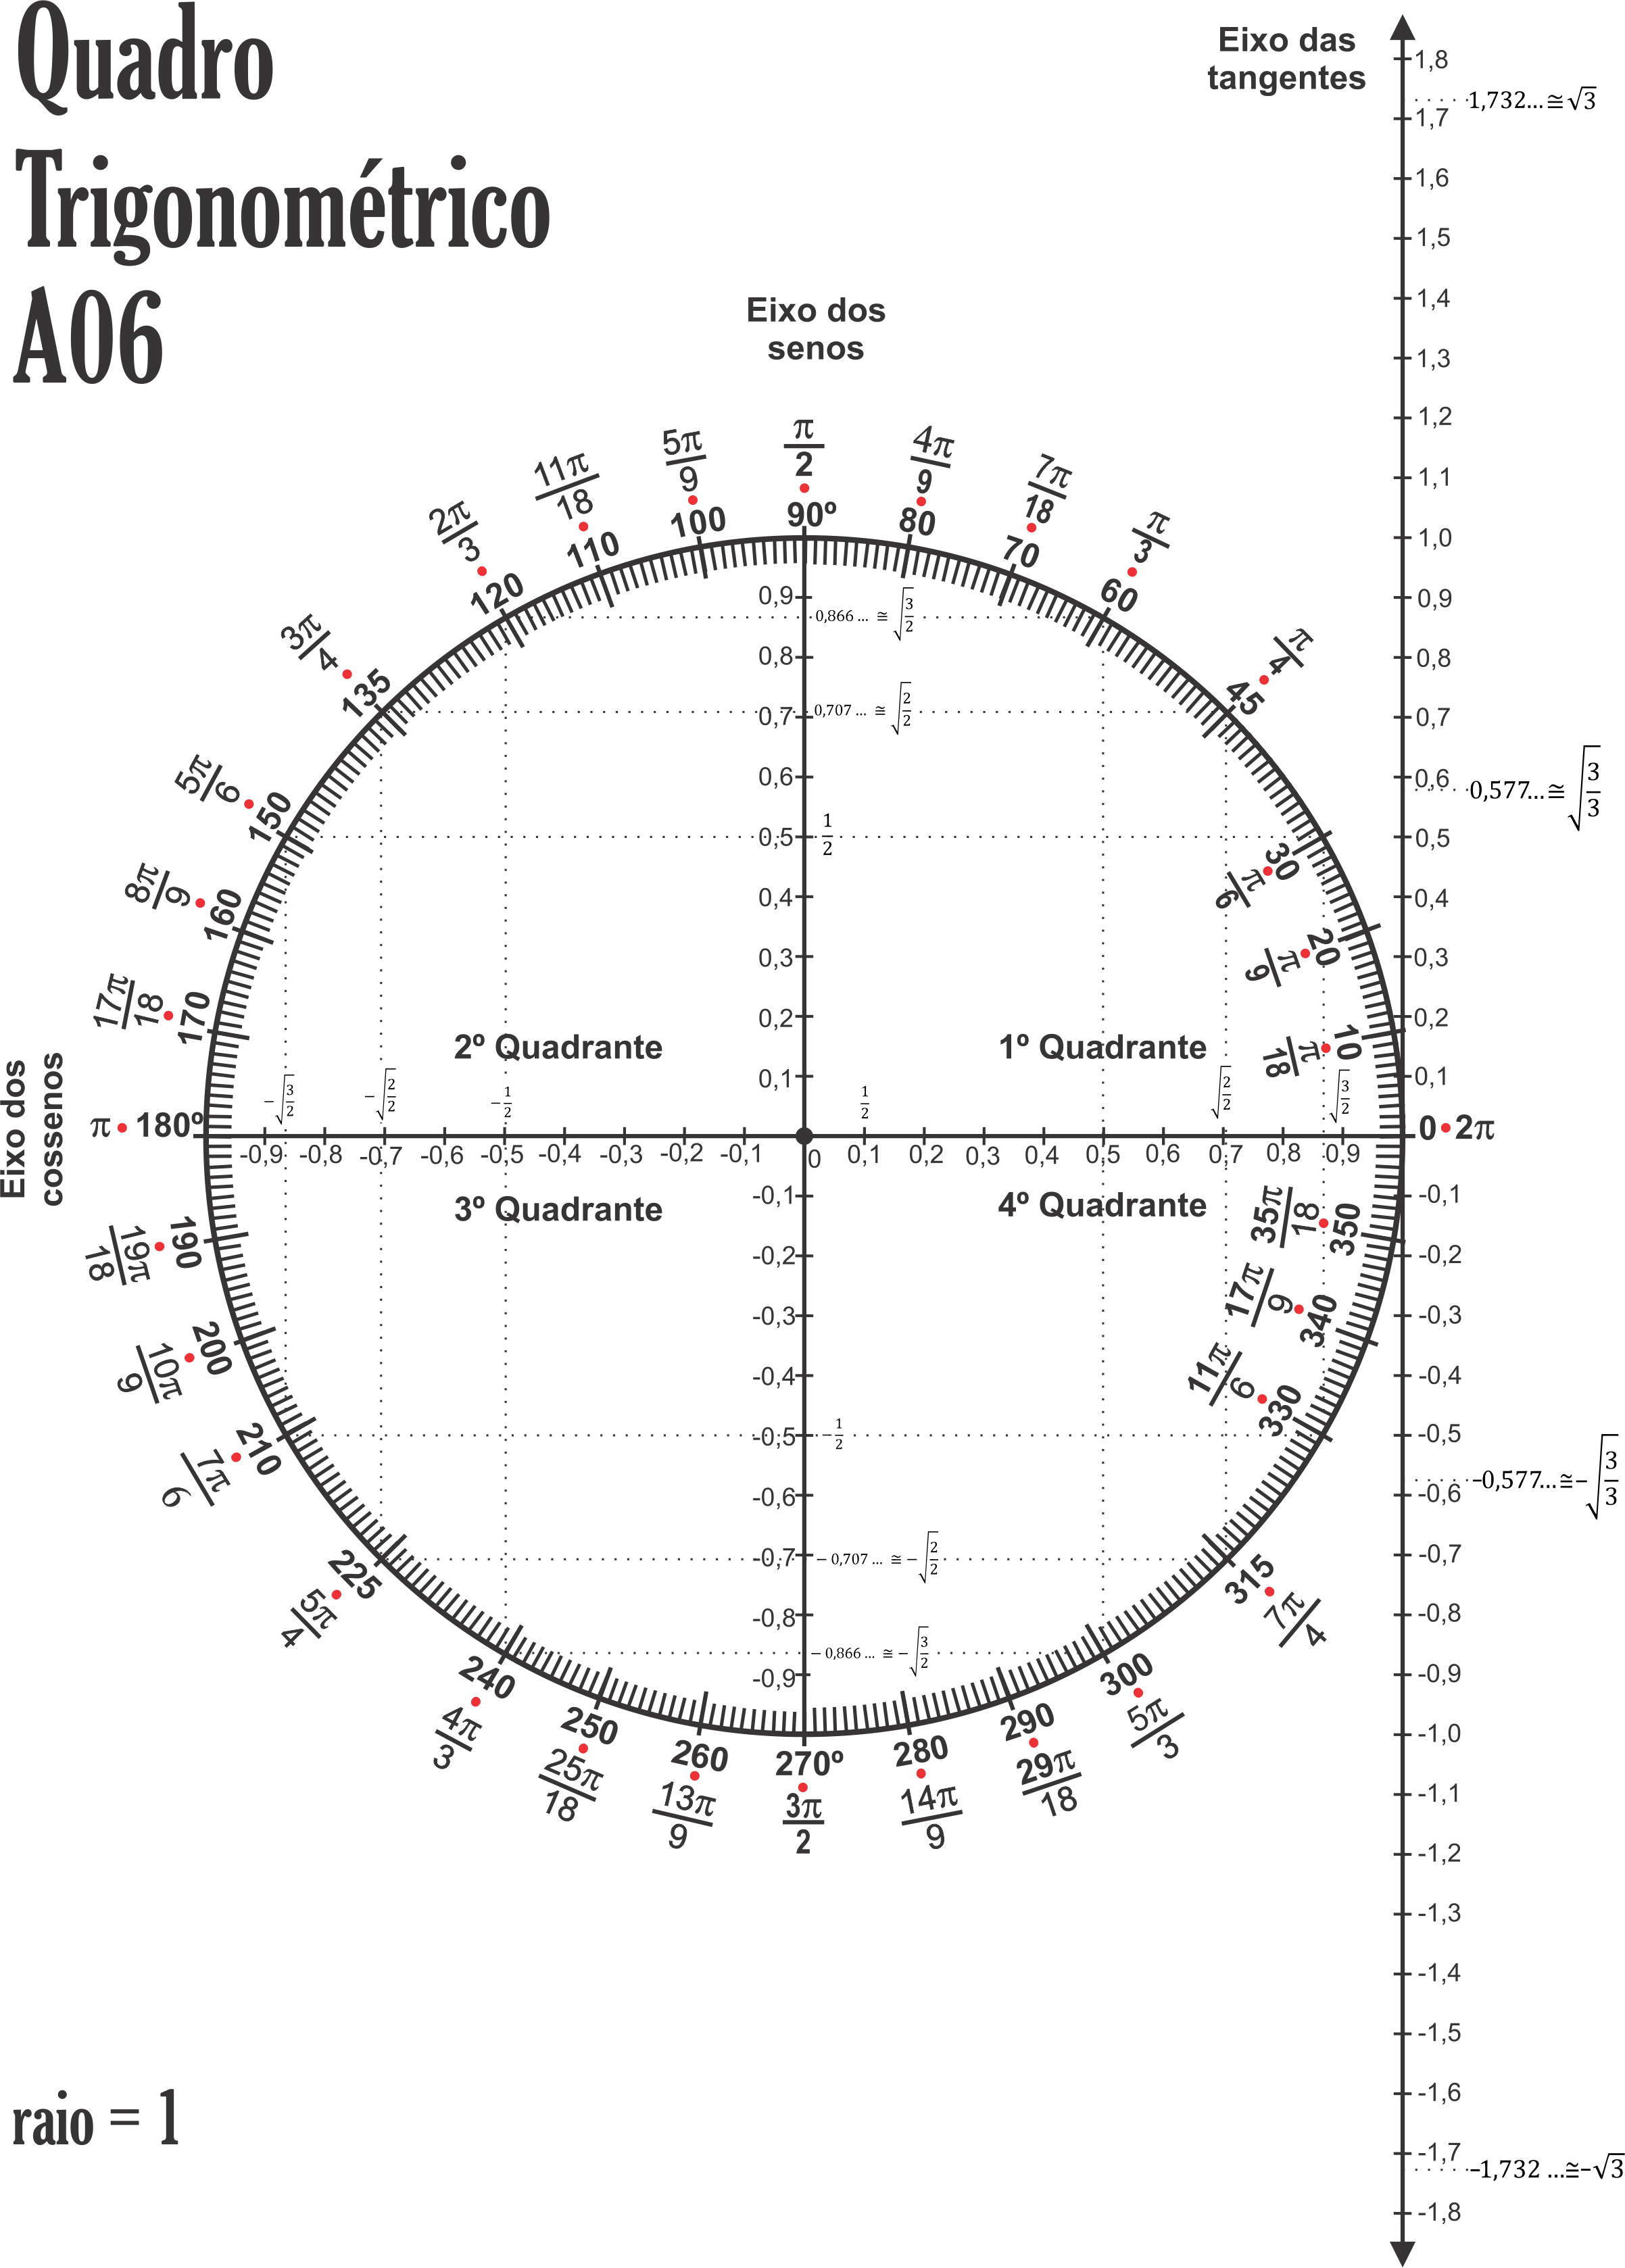
\includegraphics[width=0.9\linewidth]{chapters/appendixLesson/Interface_A06.png}
\end{figure}